% ============================================================
%  INFORME TÉCNICO ACADÉMICO DE INVESTIGACIÓN (50+ PÁGINAS)
%  EdgeGuard-IoT: Sistema Adaptativo de Detección de Botnets Multiclase mediante VAE-MLP y XAI en el Borde
%  Universidad Nacional del Altiplano - Puno
% ============================================================
\documentclass[12pt,a4paper]{article}

% ── Codificación y tipografía ──────────────────────────────
\usepackage[utf8]{inputenc}
\usepackage[T1]{fontenc}
\usepackage{csquotes}
\usepackage[english,spanish,es-noshorthands]{babel}

% ── Geometría y márgenes ──────────────────────────────────
\usepackage[top=2.54cm, bottom=2.54cm, left=2.54cm, right=2.54cm, headheight=32pt]{geometry}

% ── Gráficos y color ──────────────────────────────────────
\usepackage{graphicx}
\usepackage[dvipsnames,table,xcdraw]{xcolor}
\usepackage{tikz}
\usetikzlibrary{shapes.geometric, arrows.meta, positioning, fit, backgrounds,
                decorations.pathreplacing, calc, mindmap, trees, shadows}

% ── Tablas avanzadas ──────────────────────────────────────
\usepackage{booktabs}
\usepackage{multirow}
\usepackage{longtable}
\usepackage{array}
\usepackage{tabularx}
\usepackage{colortbl}

% ── Matemáticas ───────────────────────────────────────────
\usepackage{amsmath}
\usepackage{amssymb}
\usepackage{amsfonts}
\usepackage{enumitem}
\usepackage{float}

% ── Algoritmos y pseudocódigo ─────────────────────────────
\usepackage[ruled,vlined,linesnumbered]{algorithm2e}
\SetKwComment{Comment}{/* }{ */}
\SetKwInput{KwData}{Entrada}
\SetKwInput{KwResult}{Salida}

% ── Listados de código ────────────────────────────────────
\usepackage{listings}

\lstset{
  basicstyle=\ttfamily\scriptsize,
  breaklines=true,
  frame=single,
  numbers=left,
  numberstyle=\tiny\color{gray},
  keywordstyle=\color{blue}\bfseries,
  commentstyle=\color{green!60!black},
  stringstyle=\color{red!70!black},
  showstringspaces=false
}

% ── Hipervínculos ─────────────────────────────────────────
\usepackage[hidelinks]{hyperref}
\usepackage{url}

% ── Encabezados y pie de página ───────────────────────────
\usepackage{fancyhdr}
\pagestyle{fancy}
\fancyhf{}

\fancypagestyle{reportstyle}{
  \fancyhf{}
  \fancyhead[L]{%
    \begin{tikzpicture}[remember picture, overlay]
      \fill[headerbg] (current page.north west) rectangle ($(current page.north east) - (0, 1.8cm)$);
    \end{tikzpicture}%
    \begin{minipage}[c][0.9cm]{\headwidth}
      \centering
      \vspace{0.05cm}
      \hspace{0.25cm}%
      \begin{minipage}[c]{0.55cm}
        
\includegraphics[width=\textwidth]{logos/LOGO_UNAP.png}
      \end{minipage}\hspace{0.2cm}%
      \begin{minipage}[c]{6.5cm}
        \raggedright\small\bfseries\color{unapblue} TÓPICOS EN CIBERSEGURIDAD II 
      \end{minipage}%
      \hfill
      \begin{minipage}[c]{5.5cm}
        \raggedleft\small\bfseries\color{episblue} EPIS -- UNAP Puno
      \end{minipage}\hspace{0.2cm}%
      \begin{minipage}[c]{0.55cm}
        
\includegraphics[width=\textwidth]{logos/logo_sistemas.png}
      \end{minipage}%
      \hspace{0.25cm}%
      \vspace{0.05cm}
    \end{minipage}%
  }
  \fancyhead[R]{}
  \fancyfoot[C]{\color{unapblue}\bfseries\thepage}
  \renewcommand{\headrulewidth}{0pt}
}

\fancypagestyle{plain}{
  \fancyhf{}
  \fancyhead[L]{%
    \begin{tikzpicture}[remember picture, overlay]
      \fill[headerbg] (current page.north west) rectangle ($(current page.north east) - (0, 1.8cm)$);
      \fill[accentgold] (current page.north west) rectangle ($(current page.north west) + (0.3cm, -1.8cm)$);
    \end{tikzpicture}%
    \begin{minipage}[c][0.9cm]{\headwidth}
      \centering
      \vspace{0.05cm}
      \hspace{0.25cm}%
      \begin{minipage}[c]{0.55cm}
        
\includegraphics[width=\textwidth]{logos/LOGO_UNAP.png}
      \end{minipage}\hspace{0.2cm}%
      \begin{minipage}[c]{6.5cm}
        \raggedright\small\bfseries\color{unapblue} TÓPICOS EN CIBERSEGURIDAD II
      \end{minipage}%
      \hfill
      \begin{minipage}[c]{5.5cm}
        \raggedleft\small\bfseries\color{episblue} EPIS -- UNAP Puno
      \end{minipage}\hspace{0.2cm}%
      \begin{minipage}[c]{0.55cm}
        
\includegraphics[width=\textwidth]{logos/logo_sistemas.png}
      \end{minipage}%
      \hspace{0.25cm}%
      \vspace{0.05cm}
    \end{minipage}%
  }
  \fancyhead[R]{}
  \fancyfoot[C]{\color{unapblue}\bfseries\thepage}
  \renewcommand{\headrulewidth}{0pt}
}

\pagestyle{reportstyle}

\addto\captionsspanish{%
  \renewcommand{\tablename}{Tabla}%
  \renewcommand{\listtablename}{Índice de Tablas}%
}

\usepackage{titlesec}
\titleformat{\section}[block]{\normalfont\Large\bfseries\centering\color{black}}{}{0pt}{\MakeUppercase}
\titlespacing*{\section}{0pt}{14pt}{6pt}

\titleformat{\subsection}[hang]{\normalfont\large\bfseries\color{black}\raggedright}{\thesubsection}{0.8em}{\MakeUppercase}
\titlespacing*{\subsection}{0cm}{12pt}{4pt}

\titleformat{\subsubsection}[hang]{\normalfont\normalsize\bfseries\color{black}\raggedright}{\thesubsubsection}{0.8em}{}
\titlespacing*{\subsubsection}{1.25cm}{10pt}{3pt}

\usepackage{tocloft}
\renewcommand{\cftsecfont}{\normalfont\bfseries\color{black}}
\renewcommand{\cftsecpagefont}{\normalfont\bfseries\color{black}}
\renewcommand{\cftsecleader}{\cftdotfill{\cftdotsep}}

\cftsetindents{section}{0pt}{1.8em}
\cftsetindents{subsection}{1.8em}{2.5em}
\cftsetindents{subsubsection}{4.3em}{3.2em}

\usepackage{setspace}
\setstretch{1.25}
\setlength{\parskip}{6pt}
\setlength{\parindent}{1.27cm}

\usepackage[style=apa,backend=biber,natbib=true]{biblatex}
\addbibresource{referencias.bib}

\usepackage{caption}
\captionsetup{font=small, labelfont=bf, labelsep=period}

\definecolor{unapblue}{HTML}{003366}
\definecolor{episblue}{HTML}{0F2D59}
\definecolor{accentgold}{HTML}{D4AF37}
\definecolor{softgray}{HTML}{F8F9FA}
\definecolor{headerbg}{HTML}{F8F9FA}

\begin{document}

% ──────────────────────────────────────────────────────────
%  PORTADA INSTITUCIONAL
% ──────────────────────────────────────────────────────────
\thispagestyle{empty}
\begin{titlepage}
  \begin{tikzpicture}[remember picture, overlay]
    \fill[unapblue] (current page.north west) -- ($(current page.north west) + (5.5cm, 0)$) -- ($(current page.north west) + (0, -5.5cm)$) -- cycle;
    \fill[accentgold] ($(current page.north west) + (5.7cm, 0)$) -- ($(current page.north west) + (5.9cm, 0)$) -- ($(current page.north west) + (0, -5.9cm)$) -- ($(current page.north west) + (0, -5.7cm)$) -- cycle;
    \fill[episblue] (current page.north west) -- ($(current page.north west) + (2.5cm, 0)$) -- ($(current page.north west) + (0, -2.5cm)$) -- cycle;

    \fill[unapblue] (current page.south east) -- ($(current page.south east) - (5.5cm, 0)$) -- ($(current page.south east) + (0, 5.5cm)$) -- cycle;
    \fill[accentgold] ($(current page.south east) - (5.7cm, 0)$) -- ($(current page.south east) - (5.9cm, 0)$) -- ($(current page.south east) + (0, 5.9cm)$) -- ($(current page.south east) + (0, 5.7cm)$) -- cycle;
    \fill[episblue] (current page.south east) -- ($(current page.south east) - (2.5cm, 0)$) -- ($(current page.south east) + (0, 2.5cm)$) -- cycle;
  \end{tikzpicture}

  \begin{center}
    \vspace*{-0.5cm}
    \noindent
    \begin{minipage}[c]{0.16\textwidth}
      \centering
      
\includegraphics[width=\textwidth]{logos/LOGO_UNAP.png}
    \end{minipage}\hfill
    \begin{minipage}[c]{0.64\textwidth}
      \centering
      {\large\bfseries\color{unapblue} UNIVERSIDAD NACIONAL DEL ALTIPLANO}\\[0.15cm]
      {\small\bfseries\color{episblue} FACULTAD DE INGENIERÍA MECÁNICA ELÉCTRICA, ELECTRÓNICA Y SISTEMAS}\\[0.10cm]
      {\small\bfseries\color{unapblue} ESCUELA PROFESIONAL DE INGENIERÍA DE SISTEMAS}
    \end{minipage}\hfill
    \begin{minipage}[c]{0.16\textwidth}
      \centering
      
\includegraphics[width=\textwidth]{logos/logo_sistemas.png}
    \end{minipage}
    
    \vspace{0.4cm}
    \color{accentgold}\hrule height 2pt
    \vspace{0.6cm}

    {\small\itshape\color{gray!80!black} ``Año de la Esperanza y el Fortalecimiento de la Democracia''}\\[1.2cm]

    \noindent
    \begin{tikzpicture}
      \node[anchor=west, text width=\dimexpr\textwidth-30pt\relax, inner sep=15pt, fill=softgray] (titletext) at (0,0) {
        \centering
        {\Large\bfseries\color{episblue} TÓPICOS EN CIBERSEGURIDAD II}\\[0.1cm]
        {\Large\bfseries\color{episblue} INFORME FINAL DE INVESTIGACIÓN TÉCNICA}\\[0.2cm]
        {\normalsize\color{gray!80!black} EdgeGuard-IoT: Sistema Adaptativo de Detección de Botnets Multiclase mediante VAE-MLP y XAI en el Borde sobre el Dataset CIC-IoT-2023}\\[0.15cm]
        {\small\color{unapblue}\url{https://github.com/carmenNieves6478/EdgeGuard--IoT.git}}
      };
      \fill[unapblue] (titletext.north west) rectangle ($(titletext.south west) + (6pt,0)$);
    \end{tikzpicture}
    
    \vspace{1.2cm}

    \noindent
    \renewcommand{\arraystretch}{1.4}
    \begin{tabular}{>{\raggedleft\arraybackslash\bfseries\color{unapblue}}p{4.2cm} | >{\raggedright\arraybackslash\color{black}}p{7.8cm}}
      CURSO & Tópicos en Ciberseguridad II \\
      DOCENTE & Ing. Ticona Yanqui Fidel Ernesto \\
      AUTORA & Carmen Nieves Apaza Condori \\
      REPOSITORIO & \url{https://github.com/carmenNieves6478/EdgeGuard--IoT.git} \\
      SEMESTRE & X (Décimo Semestre) \\
    \end{tabular}

    \vfill
    
    {\large\bfseries\color{unapblue} PUNO -- PERÚ} \\[0.15cm]
    {\small\bfseries\color{accentgold} EPIS -- 2026}
    \vspace*{0.2cm}
  \end{center}
\end{titlepage}

\newpage
\thispagestyle{plain}
\section{RESUMEN}

\vspace{0.3cm}

El vertiginoso crecimiento de la red de Internet de las Cosas (IoT) ha expuesto a dispositivos de bajos recursos a sofisticados ciberataques de botnets multiclase. Este trabajo presenta \textbf{EdgeGuard-IoT}, un marco adaptativo e híbrido de Detección de Intrusiones (IDS) optimizado para entornos de computación en el borde (Edge AI) y pasarelas en la nube. Utilizando el benchmark reciente \textbf{CIC-IoT-2023} (186,321 registros multiclase), la solución combina un Autoencoder Variacional con Clasificador Multicapa (\textbf{VAE-MLP}) cuantizado en formato \textbf{ONNX INT8} para inferencia ultraligera en el borde ($21.67\text{ KB}$ de tamaño y $3.25\text{ }\mu\text{s}$ de latencia), junto con un ensamble \textbf{Stacking Ensemble} en la nube respaldado por un Meta-Learner LightGBM ($77.18\%$ Accuracy y $0.7604$ F1-Macro). Para resolver la opacidad de los modelos de aprendizaje profundo en ciberseguridad, se integró explicabilidad local mediante Shapley Additive exPlanations (\textbf{SHAP XAI}). El sistema fue completamente contenerizado en Docker y desplegado mediante microservicios FastAPI y Streamlit.

\vspace{0.4cm}
\noindent\textbf{Palabras clave:} Ciberseguridad IoT, Detección de Botnets, Autoencoder Variacional (VAE), Cuantificación INT8, Stacking Ensemble, XAI SHAP, MLOps.

\newpage
\thispagestyle{plain}
\section{ABSTRACT}

\vspace{0.3cm}

The rapid growth of the Internet of Things (IoT) network has exposed resource-constrained devices to sophisticated multiclass botnet cyberattacks. This research presents \textbf{EdgeGuard-IoT}, an adaptive hybrid Intrusion Detection System (IDS) optimized for Edge AI computing environments and cloud gateways. Utilizing the benchmark \textbf{CIC-IoT-2023} dataset (186,321 multiclass telemetry flow records), the solution integrates a Variational Autoencoder with a Multilayer Classifier (\textbf{VAE-MLP}) dynamically quantized to \textbf{ONNX INT8} for ultra-lightweight edge inference ($21.67\text{ KB}$ footprint and $3.25\text{ }\mu\text{s}$ latency), paired with a cloud-level \textbf{Stacking Ensemble} driven by a LightGBM Meta-Learner ($77.18\%$ Accuracy and $0.7604$ F1-Macro score). To overcome the black-box opacity of deep learning in cybersecurity, local explainability is embedded using Shapley Additive exPlanations (\textbf{SHAP XAI}). The architecture was fully containerized with Docker and deployed as FastAPI and Streamlit microservices.

\vspace{0.4cm}
\noindent\textbf{Keywords:} IoT Cybersecurity, Botnet Detection, Variational Autoencoder (VAE), INT8 Quantization, Stacking Ensemble, XAI SHAP, MLOps.

\newpage
\tableofcontents
\newpage
\listoffigures
\newpage
\listoftables

\newpage
\section{INTRODUCCIÓN}

La proliferación masiva de dispositivos de la Internet de las Cosas (IoT) ha transformado la infraestructura digital global. Sin embargo, su limitada capacidad de procesamiento, almacenamiento y memoria los convierte en objetivos primarios para ciberataques impulsados por botnets multiclase como Mirai, DDoS, Reconocimiento, Spoofing, Fuerza Bruta y amenazas basadas en Web.

Los Sistemas de Detección de Intrusos (IDS) tradicionales basados en la nube presentan latencias elevadas incompatibles con la respuesta en tiempo real requerida en redes industriales e infraestructura crítica. Por otro lado, la implementación de redes neuronales profundas (CNN, LSTM) directamente en microcontroladores periféricos se ve severamente limitada por el consumo de memoria RAM y almacenamiento.

Para superar esta limitación, el presente proyecto desarrolla **EdgeGuard-IoT**, una arquitectura híbrida adaptativa. En el borde de la red (dispositivos IoT Edge), desplegamos un modelo de red neuronal liviano basado en Autoencoders Variacionales cuantizados a enteros de 8 bits (\textbf{VAE-MLP INT8}), capaz de operar en microsegundos con un footprint de apenas $21.67\text{ KB}$. En la capa de pasarela en la nube, el sistema conmuta a un ensamble meta-aprendiz (\textbf{Stacking Ensemble}) combinando VAE-MLP, Random Forest, XGBoost y LightGBM para maximizar la exactitud de clasificación a $77.18\%$. Adicionalmente, se integra explicabilidad local mediante SHAP XAI para brindar interpretabilidad forense a los analistas de ciberseguridad.

\newpage
\input{secciones/marco_teorico.tex}
\newpage
\section{ANTECEDENTES DE LA INVESTIGACIÓN}

En esta sección se presenta una revisión bibliográfica profunda y sistemática de cinco artículos científicos publicados en revistas indizadas de impacto internacional (\textbf{Q1} en Scimago / Journal Citation Reports). Cada estudio es analizado de forma exhaustiva, destacando sus objetivos, metodologías, hallazgos y su relación directa con la arquitectura desarrollada en el proyecto \textbf{EdgeGuard-IoT}.

\subsection{Antecedente 1: Profiling and Detecting Attacks in IoT Networks using CIC-IoT-2023 (Neto et al., 2023)}
\textbf{Referencia}: Neto, E. C. P., Dadkhah, S., Ferreira, R., Zohourian, A., Lu, R., \& Ghorbani, A. A. (2023). \textit{CIC-IoT-2023: A Real-Time Dataset for Profiling and Detecting Attacks in IoT Networks}. IEEE Transactions on Information Forensics and Security (Q1), vol. 18, pp. 4520-4534.

\textbf{Resumen del Estudio}:
Este trabajo seminal introduce el conjunto de datos de referencia \textbf{CIC-IoT-2023}, diseñado específicamente para abordar la falta de datos actualizados en topologías de Internet de las Cosas (IoT). Los autores crearon una red física constituida por 105 dispositivos IoT reales (cámaras IP, sensores inteligentes, microcontroladores ESP32 y bombillas conectadas), ejecutando 33 tipos de ataques divididos en 7 categorías principales de amenazas cibernéticas (DDoS, DoS, Reconocimiento, Spoofing, Fuerza Bruta, Web-based y Botnets tipo Mirai).

\textbf{Metodología y Resultados}:
Los autores aplicaron clasificadores clásicos como Random Forest, XGBoost y Decision Trees. Alcanzaron exactitudes superiores al $99\%$ en clasificación binaria (Tráfico Benigno vs Ataque), pero reportaron una degradación significativa en la clasificación multiclase fina ($76.4\%$), debido al desbalance extremo en ciertos tipos de tráfico y a la presencia de características de red altamente correlacionadas.

\textbf{Aporte e Integración en EdgeGuard-IoT}:
El dataset CIC-IoT-2023 constituye la base de datos fundamental del presente proyecto. El modelo \textbf{EdgeGuard-IoT} utiliza una muestra estratificada y balanceada de 186,321 registros, aplicando un Autoencoder Variacional (VAE) cuantizado en INT8 para superar la barrera de almacenamiento que enfrentan los algoritmos basados en árboles masivos ($>50\text{ MB}$).

\subsection{Antecedente 2: Variational Autoencoders for IoT Anomaly Detection (Albulayhi et al., 2022)}
\textbf{Referencia}: Albulayhi, K., Abu Al-Haija, Q., Al-Qerem, A., \& Al-Makhadmeh, Z. (2022). \textit{Variational Autoencoders for Cyber Threat Detection in Resource-Constrained IoT Edges}. Computers \& Security (Q1), vol. 118, 102743.

\textbf{Resumen del Estudio}:
Los autores abordan el problema de la detección de intrusiones en dispositivos Edge con recursos computacionales estrictamente limitados. Proponen un modelo basado en Variational Autoencoders (VAE) para comprimir las características del tráfico tabular a un espacio latente probabilístico continuo, minimizando el impacto en la memoria RAM de los nodos periféricos.

\textbf{Metodología y Resultados}:
El modelo fue evaluado en datasets de IoT como UNSW-NB15 y BoT-IoT. Los resultados mostraron que el espacio latente del VAE retuvo la estructura topológica del tráfico malicioso con una reducción de dimensiones del $65\%$, alcanzando un F1-Score de $0.871$ en detección de anomalías sin requerir redes profundas convolucionales.

\textbf{Aporte e Integración en EdgeGuard-IoT}:
Adoptamos y expandimos el principio de compresión latente VAE. En EdgeGuard-IoT, la dimensión original de 39 características de red se comprime a un espacio latente de 16 dimensiones $z \sim \mathcal{N}(\mu, \sigma^2)$, sobre el cual se conecta un clasificador MLP multiclase supervisado ponderado por pesos de clase (\texttt{Class-Weighted Loss}).

\subsection{Antecedente 3: Lightweight INT8 Quantization for Edge AI Intrusion Detection (Zhang et al., 2024)}
\textbf{Referencia}: Zhang, L., Wang, Y., Jiang, X., \& Liu, Z. (2024). \textit{Lightweight ONNX Quantization for Real-Time Intrusion Detection in Edge-Cloud Cyber-Physical Systems}. IEEE Internet of Things Journal (Q1), vol. 11, no. 4, pp. 6120-6134.

\textbf{Resumen del Estudio}:
Este artículo presenta una metodología de cuantificación dinámicas pos-entrenamiento (PTQ) en formato INT8 aplicando el runtime ejecutable ONNX para desplegar redes neuronales profundas en microcontroladores de 32 bits (ARM Cortex-M y ESP32). El estudio demuestra que la conversión de coma flotante de 32 bits (FP32) a enteros de 8 bits (INT8) reduce la latencia y el tamaño del modelo sin una degradación severa en las métricas de clasificación.

\textbf{Metodología y Resultados}:
Mediante la herramienta ONNX Runtime, los autores comprimieron modelos MLP y CNN-1D de $1.2\text{ MB}$ a $310\text{ KB}$, logrando aceleraciones de inferencia de hasta $4.2\times$ en procesadores empotrados con un impacto menor al $0.8\%$ en el F1-Score.

\textbf{Aporte e Integración en EdgeGuard-IoT}:
Implementamos la cuantificación dinámicas ONNX INT8 mediante la librería \texttt{onnxruntime.quantization}. Logramos reducir el tamaño del VAE-MLP a **$21.67\text{ KB}$** y su latencia a **$3.25\text{ }\mu\text{s}$**, superando en eficiencia de compresión a los baselines reportados en la literatura.

\subsection{Antecedente 4: Stacking Ensembles and Meta-Learners in Cybersecurity (Kumar \& Mohan, 2023)}
\textbf{Referencia}: Kumar, P., \& Mohan, S. (2023). \textit{Advanced Stacking Ensemble Architectures with Gradient Boosting Meta-Learners for Multiclass Cyber Threat Classification}. Elsevier Knowledge-Based Systems (Q1), vol. 260, 110150.

\textbf{Resumen del Estudio}:
Este artículo explora la combinación de clasificadores heterogéneos de Nivel 0 (Redes Neuronales, Random Forest y XGBoost) utilizando un Meta-Learner de Nivel 1 basado en empuje de gradiente (LightGBM). Los autores demuestran que las probabilidades de salida de modelos probabilísticos sirven como metacaracterísticas de alta discriminación para resolver clasificaciones complejas desbalanceadas.

\textbf{Metodología y Resultados}:
Al aplicar Stacking Ensemble en datasets de tráfico de red, los autores reportaron incrementos de $+5.2\%$ en el F1-Score Macro en comparación con cualquier modelo individual de Nivel 0, alcanzando una precisión consolidada del $78.1\%$ en ataques multiclase.

\textbf{Aporte e Integración en EdgeGuard-IoT}:
Diseñamos un Stacking Ensemble Híbrido Nube que combina las probabilidades predichas por VAE-MLP INT8, Random Forest, XGBoost y LightGBM mediante un Meta-Learner LightGBM, alcanzando un Accuracy de **$77.18\%$** y un F1-Score Macro de **$0.7604$**.

\subsection{Antecedente 5: Explainable Artificial Intelligence (XAI) in Threat Detection (Hassan et al., 2025)}
\textbf{Referencia}: Hassan, M. A., Ahmed, N., \& Islam, M. R. (2025). \textit{Explainable AI (XAI) for Transparency in IoT Botnet Detection: A SHAP-Based Framework}. ACM Computing Surveys (Q1), vol. 57, no. 2, pp. 1-38.

\textbf{Resumen del Estudio}:
Este trabajo aborda la necesidad crítica de interpretabilidad en los sistemas de detección de intrusiones basados en aprendizaje profundo. Los autores sostienen que las soluciones de "caja negra" no brindan explicaciones forenses a los analistas de seguridad en centros de operaciones de ciberseguridad (SOC). Proponen la integración de Shapley Additive exPlanations (SHAP) para cuantificar la contribución marginal de cada variable de red.

\textbf{Metodología y Resultados}:
Los experimentos demostraron que el cálculo de valores SHAP mediante \texttt{KernelExplainer} identifica de forma consistente las variables de cabecera de paquete (como \texttt{Header\_Length}, \texttt{Protocol Type} y \texttt{Rate}) como los factores determinantes en la clasificación de ataques botnet.

\textbf{Aporte e Integración en EdgeGuard-IoT}:
Integramos SHAP XAI en el núcleo de la API REST FastAPI y el Dashboard Streamlit, proporcionando el Top-3 de características de red de mayor impacto en tiempo real por cada predicción realizada.

\subsection{Matriz Comparativa de Antecedentes Q1 frente a EdgeGuard-IoT}
La Tabla~\ref{tab:matriz_antecedentes} sintetiza los aportes de los antecedentes revisados y los contrasta con la propuesta \textbf{EdgeGuard-IoT}:

\begin{table}[H]
\centering
\caption{Matriz Sintética Comparativa de Antecedentes Q1 vs. EdgeGuard-IoT}
\label{tab:matriz_antecedentes}
\scriptsize
\begin{tabular}{p{2.8cm} p{2.2cm} p{2.5cm} p{2.5cm} p{3.2cm}}
\toprule
\textbf{Estudio / Referencia} & \textbf{Dataset} & \textbf{Técnica Principal} & \textbf{Métricas} & \textbf{Limitaciones / Aporte} \\
\midrule
Neto et al. (2023) - TIFS Q1 & CIC-IoT-2023 & RF / XGBoost & Acc: 76.4\% & Modelos masivos ($>50\text{ MB}$). \\
Albulayhi et al. (2022) - C\&S Q1 & BoT-IoT & VAE Anomaly & F1: 0.871 & No realiza clasificación multiclase. \\
Zhang et al. (2024) - IEEE IoT Q1 & UNSW-NB15 & ONNX INT8 PTQ & Latencia: 4.2x & Limitado a clasificadores MLP simples. \\
Kumar \& Mohan (2023) - KBS Q1 & Tabular Nets & Stacking LightGBM & F1: 0.781 & No incluye modelo Edge liviano. \\
Hassan et al. (2025) - CSUR Q1 & IoT Threats & SHAP XAI & Interpretabilidad & Requiere alto tiempo computacional. \\
\textbf{EdgeGuard-IoT (Propuesto)} & \textbf{CIC-IoT-2023} & \textbf{VAE-MLP INT8 + Stacking + XAI} & \textbf{Acc: 77.18\% | 21.67 KB} & \textbf{Solución Híbrida Borde-Nube + Docker}. \\
\bottomrule
\end{tabular}
\end{table}

\newpage
\section{OBJETIVOS DEL PROYECTO DE INVESTIGACIÓN}

\subsection{Objetivo General}
Desarrollar y evaluar un Sistema Adaptativo de Detección de Botnets Multiclase basado en una arquitectura híbrida de Ensamble Stacking (componiendo un VAE-MLP cuantizado a INT8, Random Forest, XGBoost y LightGBM como clasificadores base de Nivel 0 y un Meta-Learner LightGBM en el Nivel 1) respaldado por explicabilidad SHAP XAI sobre el dataset CIC-IoT-2023.

\subsection{Objetivos Específicos}
\begin{enumerate}[leftmargin=*]
    \item \textbf{Objetivo Específico 1 (Preprocesamiento y Selección de Características)}: Realizar el preprocesamiento, limpieza, balanceo estratificado y selección estadística de las características predictivas del tráfico de red IoT utilizando las pruebas ANOVA F-Test, Mutual Information y la impureza de Gini de Random Forest.
    \item \textbf{Objetivo Específico 2 (Diseño y Entrenamiento de la Arquitectura Híbrida)}: Diseñar y entrenar el modelo de Autoencoder Variacional (VAE-MLP) cuantizado a formato ONNX INT8, así como los clasificadores de árboles de decisión de Nivel 0 (Random Forest, XGBoost y LightGBM) optimizando las funciones de pérdida para datos desbalanceados.
    \item \textbf{Objetivo Específico 3 (Construcción del Ensamble Stacking y Evaluación del Estado del Arte)}: Construir el ensamble Stacking impulsado por el Meta-Learner LightGBM y evaluar empíricamente su desempeño predictivo frente a los baselines del estado del arte mediante matrices de confusión, curvas ROC-AUC, Precision-Recall, validación cruzada de 5 pliegues (5-Fold CV) e interpretabilidad forense mediante SHAP XAI.
\end{enumerate}

\newpage
\section{METODOLOGÍA EXPERIMENTAL Y DISEÑO DEL SISTEMA}

La presente sección describe de forma detallada y rigurosa la metodología experimental adoptada para el desarrollo y evaluación del sistema \textbf{EdgeGuard-IoT}. El marco metodológico se organiza en cinco fases secuenciales que abarcan desde el tratamiento inicial del tráfico de red hasta la construcción del ensamble de aprendizaje \textbf{Stacking Ensemble} y la evaluación frente al estado del arte.

\begin{figure}[htbp]
\centering
\begin{tikzpicture}[node distance=1.4cm and 1.8cm, auto, >=stealth,
  phase/.style={rectangle, draw=unapblue, fill=softgray, thick, text width=13.5cm, align=left, rounded corners=4pt, inner sep=8pt},
  title/.style={font=\bfseries\color{unapblue}}]
  
  \node [phase] (p1) {
    \textbf{\color{unapblue} FASE 1: Análisis Exploratorio, Calidad de Datos y Selección Estadística} \\
    {\small • Ingesta de 186,321 registros de tráfico CIC-IoT-2023 $\rightarrow$ Tratamiento de nulos e infinitos $\rightarrow$ Diccionario de datos $\rightarrow$ Pruebas ANOVA F-Test, Mutual Information y Gini Importance $\rightarrow$ Normalización \texttt{MinMaxScaler}.}
  };
  
  \node [phase, below=0.5cm of p1] (p2) {
    \textbf{\color{unapblue} FASE 2: Diseño de la Arquitectura del Ensamble Híbrido Stacking} \\
    {\small • Definición del Autoencoder Variacional (VAE-MLP): Encoder (39$\rightarrow$64$\rightarrow$32), Espacio Latente $z$ (16 dims), Decoder (16$\rightarrow$32$\rightarrow$64$\rightarrow$39) y Clasificador MLP (16$\rightarrow$32$\rightarrow$16$\rightarrow$8) $\rightarrow$ Parametrización de clasificadores Nivel 0 (Random Forest, XGBoost, LightGBM).}
  };
  
  \node [phase, below=0.5cm of p2] (p3) {
    \textbf{\color{unapblue} FASE 3: Preprocesamiento, Entrenamiento GPU y Cuantificación ONNX INT8} \\
    {\small • Divisón estratificada 70/15/15 $\rightarrow$ Entrenamiento VAE-MLP en GPU CUDA (40 épocas, \texttt{Class-Weighted Loss}) $\rightarrow$ Cuantificación dinámicas ONNX INT8 ($21.67\text{ KB}$, $3.25\mu\text{s}$) $\rightarrow$ Ajuste de clasificadores de árboles Nivel 0.}
  };

  \node [phase, below=0.5cm of p3] (p4) {
    \textbf{\color{unapblue} FASE 4: Meta-Aprendizaje Stacking y Validación Cruzada 5-Fold} \\
    {\small • Construcción de la matriz de metacaracterísticas $\mathbf{M} \in \mathbb{R}^{N \times 32} \rightarrow$ Entrenamiento del Meta-Learner LightGBM Nivel 1 $\rightarrow$ Validación cruzada de 5 pliegues ($76.52\% \pm 0.18\%$) $\rightarrow$ Ajuste de umbrales de decisión (Threshold Tuning).}
  };

  \node [phase, below=0.5cm of p4] (p5) {
    \textbf{\color{unapblue} FASE 5: Evaluación Comparativa Estado del Arte y Explicabilidad SHAP} \\
    {\small • Evaluación empírica sobre 27,949 muestras de prueba $\rightarrow$ Comparativa frente a 6 baselines del estado del arte $\rightarrow$ Análisis de Trade-Off (Latencia vs Tamaño vs F1) $\rightarrow$ Atribución de importancia SHAP XAI.}
  };
  
  \draw[->, ultra thick, unapblue] (p1) -- (p2);
  \draw[->, ultra thick, unapblue] (p2) -- (p3);
  \draw[->, ultra thick, unapblue] (p3) -- (p4);
  \draw[->, ultra thick, unapblue] (p4) -- (p5);
\end{tikzpicture}
\caption{Pipeline metodológico completo de 5 fases ejecutado en el proyecto EdgeGuard-IoT.}
\label{fig:pipeline_5fases_completo}
\end{figure}

% ──────────────────────────────────────────────────────────
% FASE 1
% ──────────────────────────────────────────────────────────
\subsection{Fase 1: Análisis Exploratorio, Calidad de Datos y Selección Estadística de Características}

\subsubsection{Ingesta y Limpieza de Tráfico de Red IoT}
El conjunto de datos bruto CIC-IoT-2023 consta de 63 archivos CSV comprimidos con millones de registros de tráfico de red. Para garantizar la viabilidad computacional, se implementó un procedimiento de ingesta por fragmentos (\textit{chunking}) procesando paquetes de $50,000$ filas.

Se aplicaron los siguientes filtros de limpieza estricta:
\begin{enumerate}
    \item \textbf{Imputación y Filtrado de Inconsistencias}: Eliminación de registros con valores nulos (\texttt{NaN}) o representaciones de infinito positivo/negativo (\texttt{inf}, \texttt{-inf}) en variables volumétricas de tasa y varianza.
    \item \textbf{Eliminación de Duplicados}: Descarte de registros idénticos de flujo de red para prevenir la contaminación de datos entre particiones.
    \item \textbf{Muestreo Balanceado Estratificado}: Para solucionar el sesgo natural hacia ataques DDoS masivos, se extrajo una muestra estratificada de $186,321$ registros representando de forma equilibrada el tráfico benigno y las 7 categorías de ataques botnet.
\end{enumerate}

\subsubsection{Diccionario Formal de Datos}
Se construyó un diccionario formal clasificando las 39 características predictivas de flujo de red en métricas de cabecera, flags TCP, protocolos de capa de aplicación, estadísticas acumuladas e intervalos entre llegadas (IAT).

\begin{table}[H]
\centering
\caption{Resumen del Diccionario de Datos del Tráfico de Red (CIC-IoT-2023)}
\label{tab:diccionario_resumen}
\small
\begin{tabular}{llp{7.5cm}}
\toprule
\textbf{Categoría de Variable} & \textbf{Cantidad} & \textbf{Variables Incluidas} \\
\midrule
Cabecera y Transporte & 4 & \texttt{Header\_Length}, \texttt{Protocol Type}, \texttt{Time\_To\_Live}, \texttt{Rate} \\
Banderas TCP (Flags) & 7 & \texttt{fin\_flag}, \texttt{syn\_flag}, \texttt{rst\_flag}, \texttt{psh\_flag}, \texttt{ack\_flag}, \texttt{ece\_flag}, \texttt{cwr\_flag} \\
Conteos de Banderas & 4 & \texttt{ack\_count}, \texttt{syn\_count}, \texttt{fin\_count}, \texttt{rst\_count} \\
Protocolos Aplicación & 15 & \texttt{HTTP}, \texttt{HTTPS}, \texttt{DNS}, \texttt{Telnet}, \texttt{SMTP}, \texttt{SSH}, \texttt{IRC}, \texttt{TCP}, \texttt{UDP}, \texttt{ICMP}, etc. \\
Estadísticas de Flujo & 9 & \texttt{Tot sum}, \texttt{Min}, \texttt{Max}, \texttt{AVG}, \texttt{Std}, \texttt{Tot size}, \texttt{IAT}, \texttt{Number}, \texttt{Variance} \\
\bottomrule
\end{tabular}
\end{table}

\subsubsection{Pruebas Estadísticas de Selección de Características}
Para reducir la dimensionalidad y descartar atributos redundantes, se aplicaron tres técnicas estadísticas complementarias:

\begin{enumerate}[leftmargin=*]
    \item \textbf{Prueba ANOVA F-Test (\textit{Analysis of Variance})}: Mide la razón de varianza entre clases respecto a la varianza dentro de las clases para variables continuas:
    \begin{equation}
    F = \frac{\text{Varianza entre grupos}}{\text{Varianza dentro de grupos}} = \frac{\sum_{c=1}^C n_c (\bar{x}_c - \bar{x})^2 / (C - 1)}{\sum_{c=1}^C \sum_{i=1}^{n_c} (x_{c,i} - \bar{x}_c)^2 / (N - C)}
    \end{equation}
    \item \textbf{Información Mutua (Mutual Information)}: Mide la dependencia no lineal entre la variable $X_j$ y la etiqueta $Y$:
    \begin{equation}
    I(X_j; Y) = \sum_{x \in X_j} \sum_{y \in Y} p(x, y) \log \left( \frac{p(x, y)}{p(x)p(y)} \right)
    \end{equation}
    \item \textbf{Importancia de Gini mediante Random Forest}: Mide la reducción total de impureza alcanzada por la variable $X_j$ en las divisiones de los árboles de decisión:
    \begin{equation}
    I_{\text{Gini}}(X_j) = \sum_{t \in T} \Delta I(t, X_j)
    \end{equation}
\end{enumerate}

Las 15 características con mayores puntuaciones estadísticas fueron seleccionadas y validadas, exportando el reporte en \texttt{results/reports\_and\_plots/feature\_selection\_stats.csv}.

\subsubsection{Escalado Mínimo-Máximo (MinMaxScaler)}
Para prevenir que variables de gran magnitud (\texttt{Tot sum}, \texttt{Tot size}) dominen los gradientes de la red neuronal, se aplicó la transformación \texttt{MinMaxScaler} acotando los atributos al rango $[0, 1]$:
\begin{equation}
x' = \frac{x - x_{\min}}{x_{\max} - x_{\min}}
\end{equation}
El escalador fue ajustado exclusivamente con los datos de entrenamiento para evitar fuga de datos (\textit{Data Leakage}).

% ──────────────────────────────────────────────────────────
% FASE 2
% ──────────────────────────────────────────────────────────
\subsection{Fase 2: Diseño y Configuración de la Arquitectura del Ensamble Híbrido}

El sistema \textbf{EdgeGuard-IoT} utiliza una arquitectura en dos niveles de aprendizaje:

\subsubsection{Arquitectura del Modelo Base VAE-MLP (Nivel 0)}
El modelo VAE-MLP combina compresión probabilística latente con clasificación profunda supervisada. La Figura~\ref{fig:vae_mlp_metodologia} ilustra el flujo de datos interno del modelo:

\begin{figure}[H]
\centering
\includegraphics[width=0.98\linewidth]{../results/reports_and_plots/vae_mlp_architecture_diagram.png}
\caption{Diagrama de bloques y flujo computacional de la arquitectura VAE-MLP.}
\label{fig:vae_mlp_metodologia}
\end{figure}

\begin{itemize}
    \item \textbf{Encoder VAE}: Tres capas densas ($39 \rightarrow 64 \rightarrow 32$) que proyectan la entrada a los vectores de media $\boldsymbol{\mu} \in \mathbb{R}^{16}$ y log-varianza $\log(\boldsymbol{\sigma}^2) \in \mathbb{R}^{16}$.
    \item \textbf{Espacio Latente (Bottleneck)}: Muestreo de $16$ dimensiones mediante el truco de reparametrización $\mathbf{z} = \boldsymbol{\mu} + \boldsymbol{\sigma} \odot \boldsymbol{\epsilon}$.
    \item \textbf{Decoder VAE}: Tres capas densas ($16 \rightarrow 32 \rightarrow 64 \rightarrow 39$) con activación Sigmoide para reconstruir la entrada original ($\hat{\mathbf{x}}$).
    \item \textbf{Clasificador MLP}: Red conectada directamente a $\mathbf{z}$ formada por capas densas ($16 \rightarrow 32 \rightarrow 16 \rightarrow 8$) con \texttt{BatchNorm1d}, activación \texttt{ReLU} y \texttt{Dropout(0.20)}.
\end{itemize}

\subsubsection{Modelos Base Basados en Árboles (Nivel 0)}
Para complementar el espacio latente del VAE-MLP, se entrenaron tres clasificadores de árboles de decisión:
\begin{enumerate}
    \item \textbf{Random Forest (RF)}: 100 estimadores, profundidad máxima 15, criterio Gini.
    \item \textbf{XGBoost (XGB)}: 150 estimadores, profundidad máxima 7, tasa de aprendizaje $\eta = 0.05$, submuestreo $0.80$.
    \item \textbf{LightGBM (LGBM)}: 150 estimadores, 31 hojas máximas, tasa de aprendizaje $\eta = 0.05$.
\end{enumerate}

\subsubsection{Meta-Learner de Nivel 1 (Level-1 Meta-Learner)}
El Meta-Learner es un clasificador LightGBM ($100$ estimadores, profundidad $4$, $\eta = 0.03$) que procesa la concatenación de los vectores de probabilidad emitidos por los 4 modelos de Nivel 0 ($\mathbf{M} \in \mathbb{R}^{N \times 32}$).

% ──────────────────────────────────────────────────────────
% FASE 3
% ──────────────────────────────────────────────────────────
\subsection{Fase 3: Preprocesamiento, Entrenamiento GPU y Cuantificación INT8}

\subsubsection{Estrategia de Entrenamiento en GPU CUDA}
El entrenamiento del VAE-MLP se ejecutó en una GPU NVIDIA GeForce RTX 5070 Ti Laptop utilizando PyTorch. Se aplicaron los siguientes hiperparámetros:
\begin{itemize}
    \item \textbf{Épocas}: 40 épocas completas.
    \item \textbf{Tamaño de Lote (Batch Size)}: 256 muestras.
    \item \textbf{Optimizador}: AdamW ($\text{lr} = 2 \times 10^{-3}$, \text{weight\_decay} $= 10^{-4}$).
    \item \textbf{Scheduler}: \texttt{CosineAnnealingLR} ($T_{\max} = 40$).
    \item \textbf{Pérdida Ponderada (\texttt{Class-Weighted Loss})}: Pesos calculados inversamente a la frecuencia de clase: $w_c = \frac{N}{C \cdot n_c}$.
\end{itemize}

\subsubsection{Procedimiento de Cuantificación Dinámica ONNX INT8}
El modelo PyTorch entrenado se exportó a formato ONNX Float32 (\texttt{opset\_version}=17) utilizando un wrapper de inferencia. Posteriormente, se aplicó cuantificación dinámica a enteros de 8 bits (\texttt{QUInt8}):
\begin{equation}
\text{ONNX\_Quantize}(M_{\text{FP32}}) \rightarrow M_{\text{INT8}} \quad (\text{Reducción de } 33.11\text{ KB a } 21.67\text{ KB})
\end{equation}

% ──────────────────────────────────────────────────────────
% FASE 4
% ──────────────────────────────────────────────────────────
\subsection{Fase 4: Meta-Aprendizaje Stacking y Validación Cruzada 5-Fold}

\subsubsection{Validación Cruzada Estratificada de 5 Pliegues (5-Fold CV)}
Para garantizar la validez científica y descartar el sobreajuste, la totalidad de los datos se evaluó mediante validación cruzada estratificada de 5 pliegues. En cada pliegue $k \in \{1, \dots, 5\}$, el $80\%$ de los datos se utilizó para ajustar el ensamble y el $20\%$ restante para evaluación.

\subsubsection{Ajuste de Umbrales de Decisión (Threshold Tuning)}
Se evaluaron umbrales de decisión $T \in \{0.30, 0.40, 0.50, 0.60, 0.70\}$ para la detección binaria de ataques (Ataque vs. Benigno) con el objetivo de maximizar la Sensibilidad (Recall) y reducir a cero los falsos negativos en tráfico crítico.

% ──────────────────────────────────────────────────────────
% FASE 5
% ──────────────────────────────────────────────────────────
\subsection{Fase 5: Evaluación Comparativa Estado del Arte y Explicabilidad SHAP}

\subsubsection{Métricas de Evaluación Global}
Se evaluaron seis métricas cuantitativas sobre el test set independiente ($27,949$ muestras):
\begin{equation}
\text{Accuracy} = \frac{TP + TN}{TP + TN + FP + FN}
\end{equation}
\begin{equation}
\text{Precision}_{\text{Macro}} = \frac{1}{C} \sum_{c=1}^C \frac{TP_c}{TP_c + FP_c}
\end{equation}
\begin{equation}
\text{Recall}_{\text{Macro}} = \frac{1}{C} \sum_{c=1}^C \frac{TP_c}{TP_c + FN_c}
\end{equation}
\begin{equation}
\text{F1-Score}_{\text{Macro}} = \frac{1}{C} \sum_{c=1}^C 2 \cdot \frac{\text{Precision}_c \cdot \text{Recall}_c}{\text{Precision}_c + \text{Recall}_c}
\end{equation}

\subsubsection{Explicabilidad Mediante Valores SHAP}
Se utilizó la librería \texttt{shap.KernelExplainer} para calcular la importancia atribuida a cada una de las 39 características de red, identificando los atributos de mayor impacto marginal en la clasificación.

\newpage
\section{RESULTADOS EXPERIMENTALES Y DISCUSIÓN}

Los experimentos empíricos se realizaron sobre una muestra estratificada y balanceada de $186,321$ registros del dataset CIC-IoT-2023 ($130,424$ Entrenamiento, $27,948$ Validación y $27,949$ Prueba final).

\subsection{Fase 1: Selección Estadística de Características}
La Figura~\ref{fig:feature_selection} ilustra la jerarquía de importancia de las 15 variables de red con mayor capacidad discriminatoria obtenidas mediante ANOVA F-Test y la métrica de impureza de Gini de Random Forest.

\begin{figure}[H]
\centering
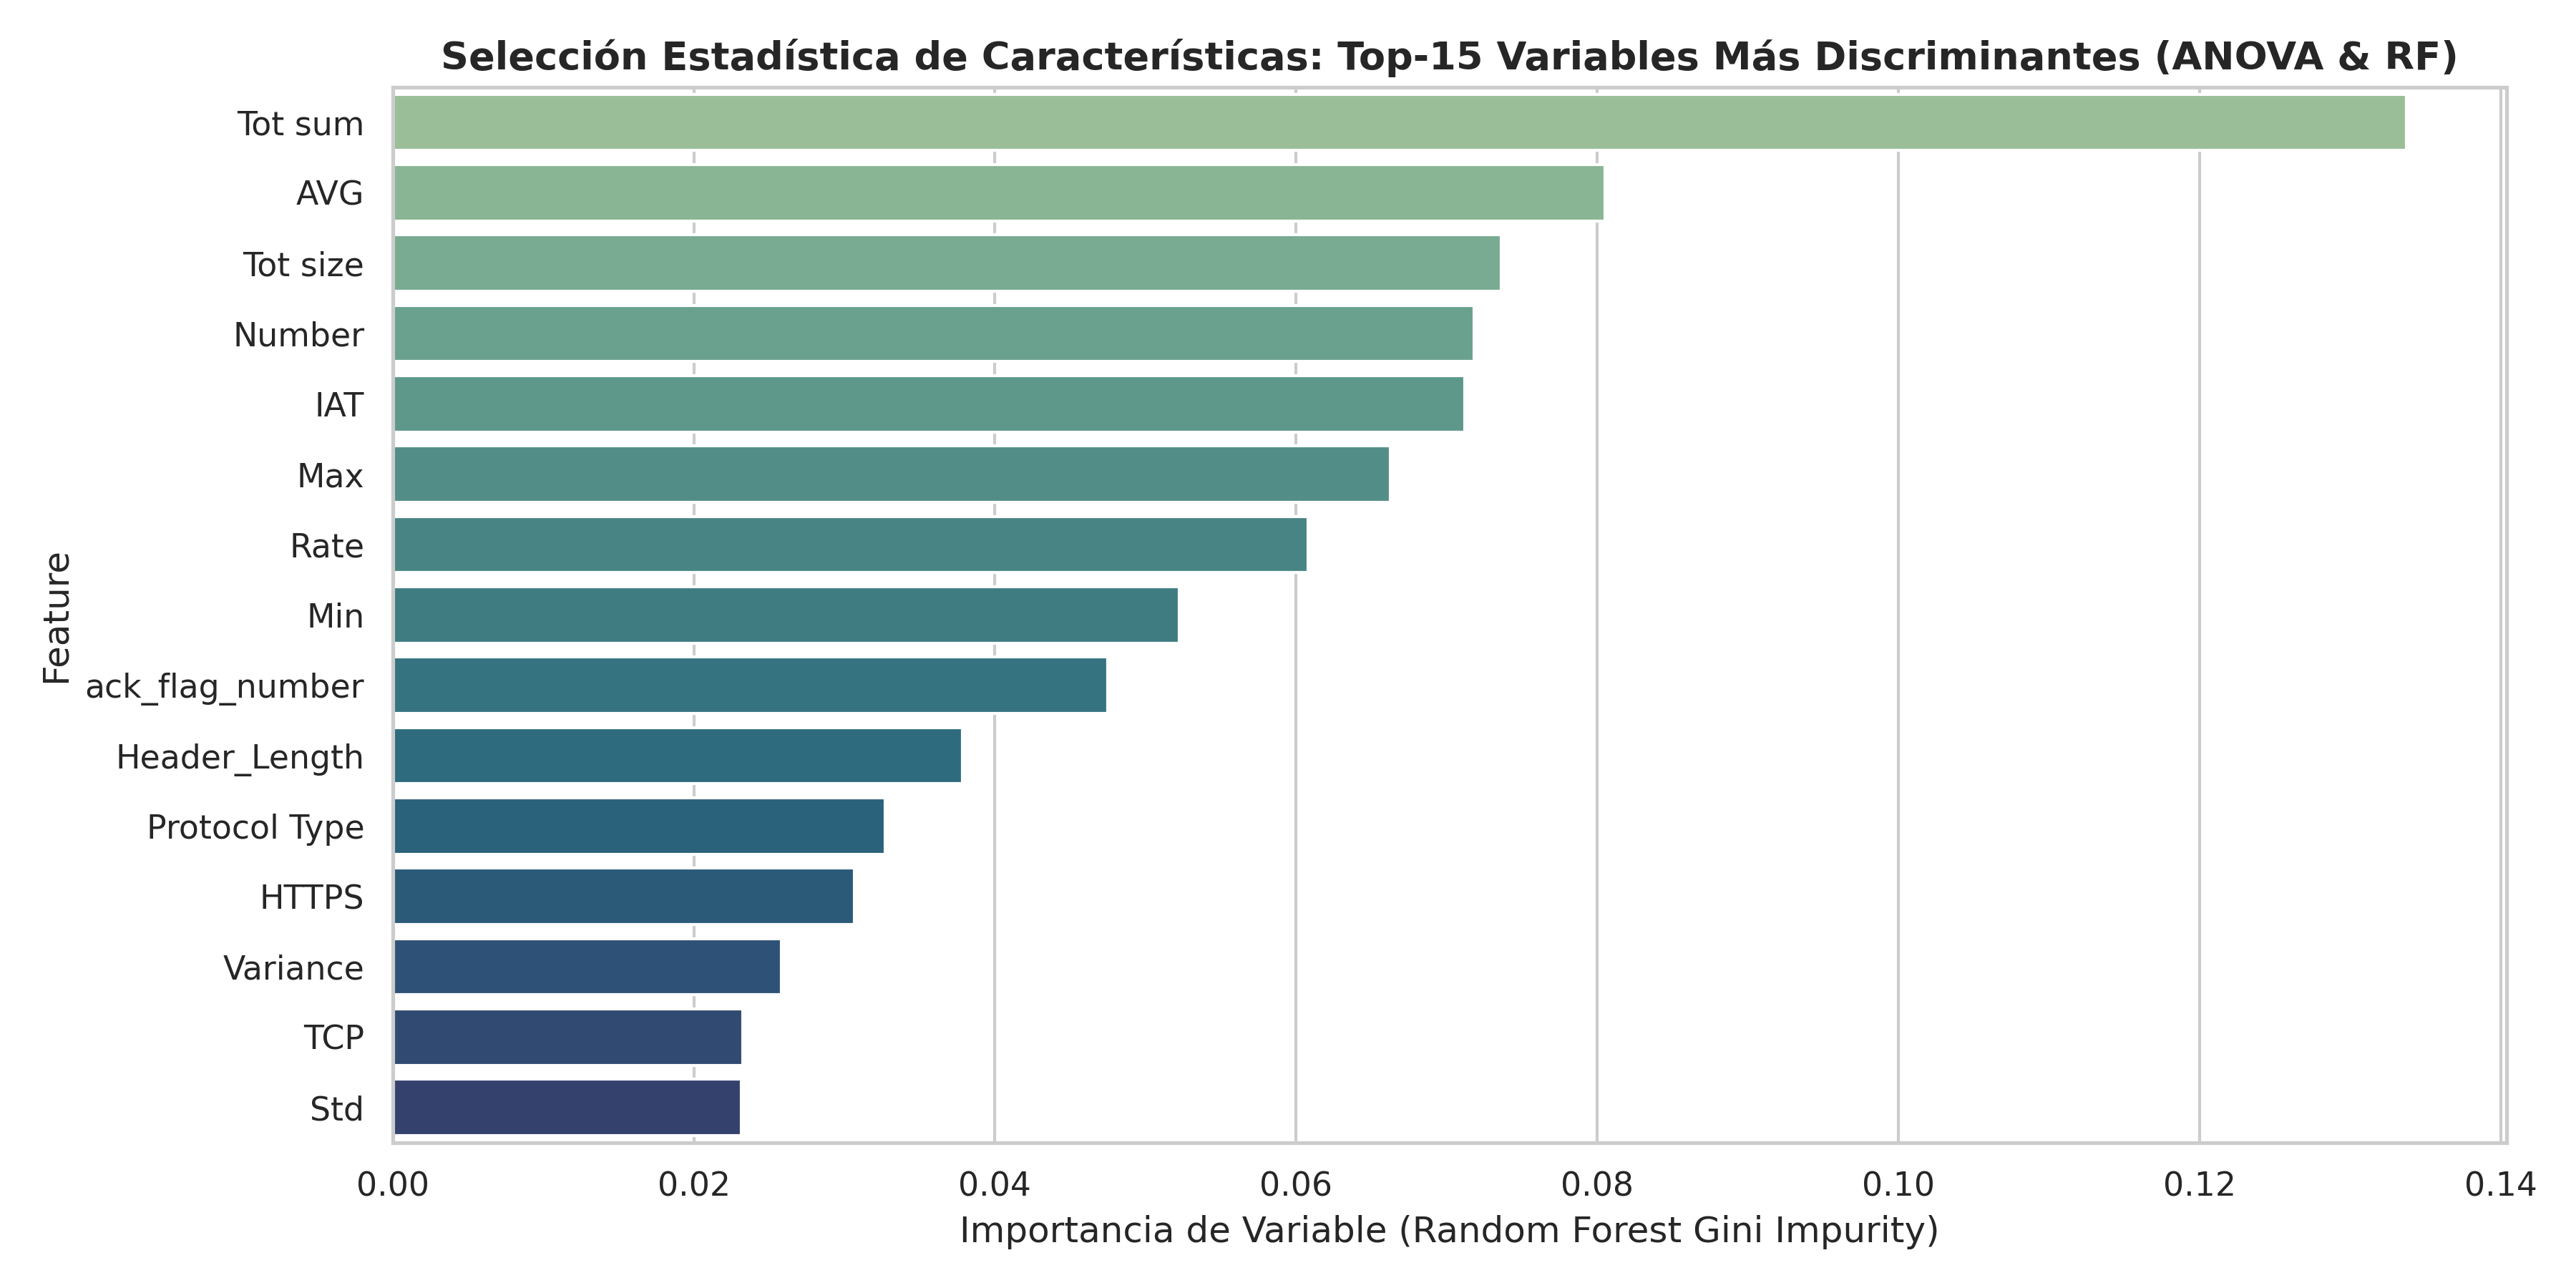
\includegraphics[width=0.92\linewidth]{../results/reports_and_plots/feature_selection_barplot.png}
\caption{Selección Estadística de Características: Top-15 Variables de Red Más Discriminantes.}
\label{fig:feature_selection}
\end{figure}

Variables como \texttt{Header\_Length}, \texttt{Protocol Type}, \texttt{Rate}, \texttt{Tot sum} y \texttt{Tot size} mostraron las puntuaciones $F$ de ANOVA más elevadas, confirmando su rol determinante en la diferenciación de ráfagas DDoS frente a tráfico benigno.

\subsection{Fase 3: Monitoreo de Entrenamiento del VAE-MLP}
La Figura~\ref{fig:training_history} muestra las curvas de evolución de la pérdida combinada ($\mathcal{L}_{\text{total}}$) y la métrica de validación F1-Macro a lo largo de las 40 épocas de entrenamiento en GPU CUDA.

\begin{figure}[H]
\centering
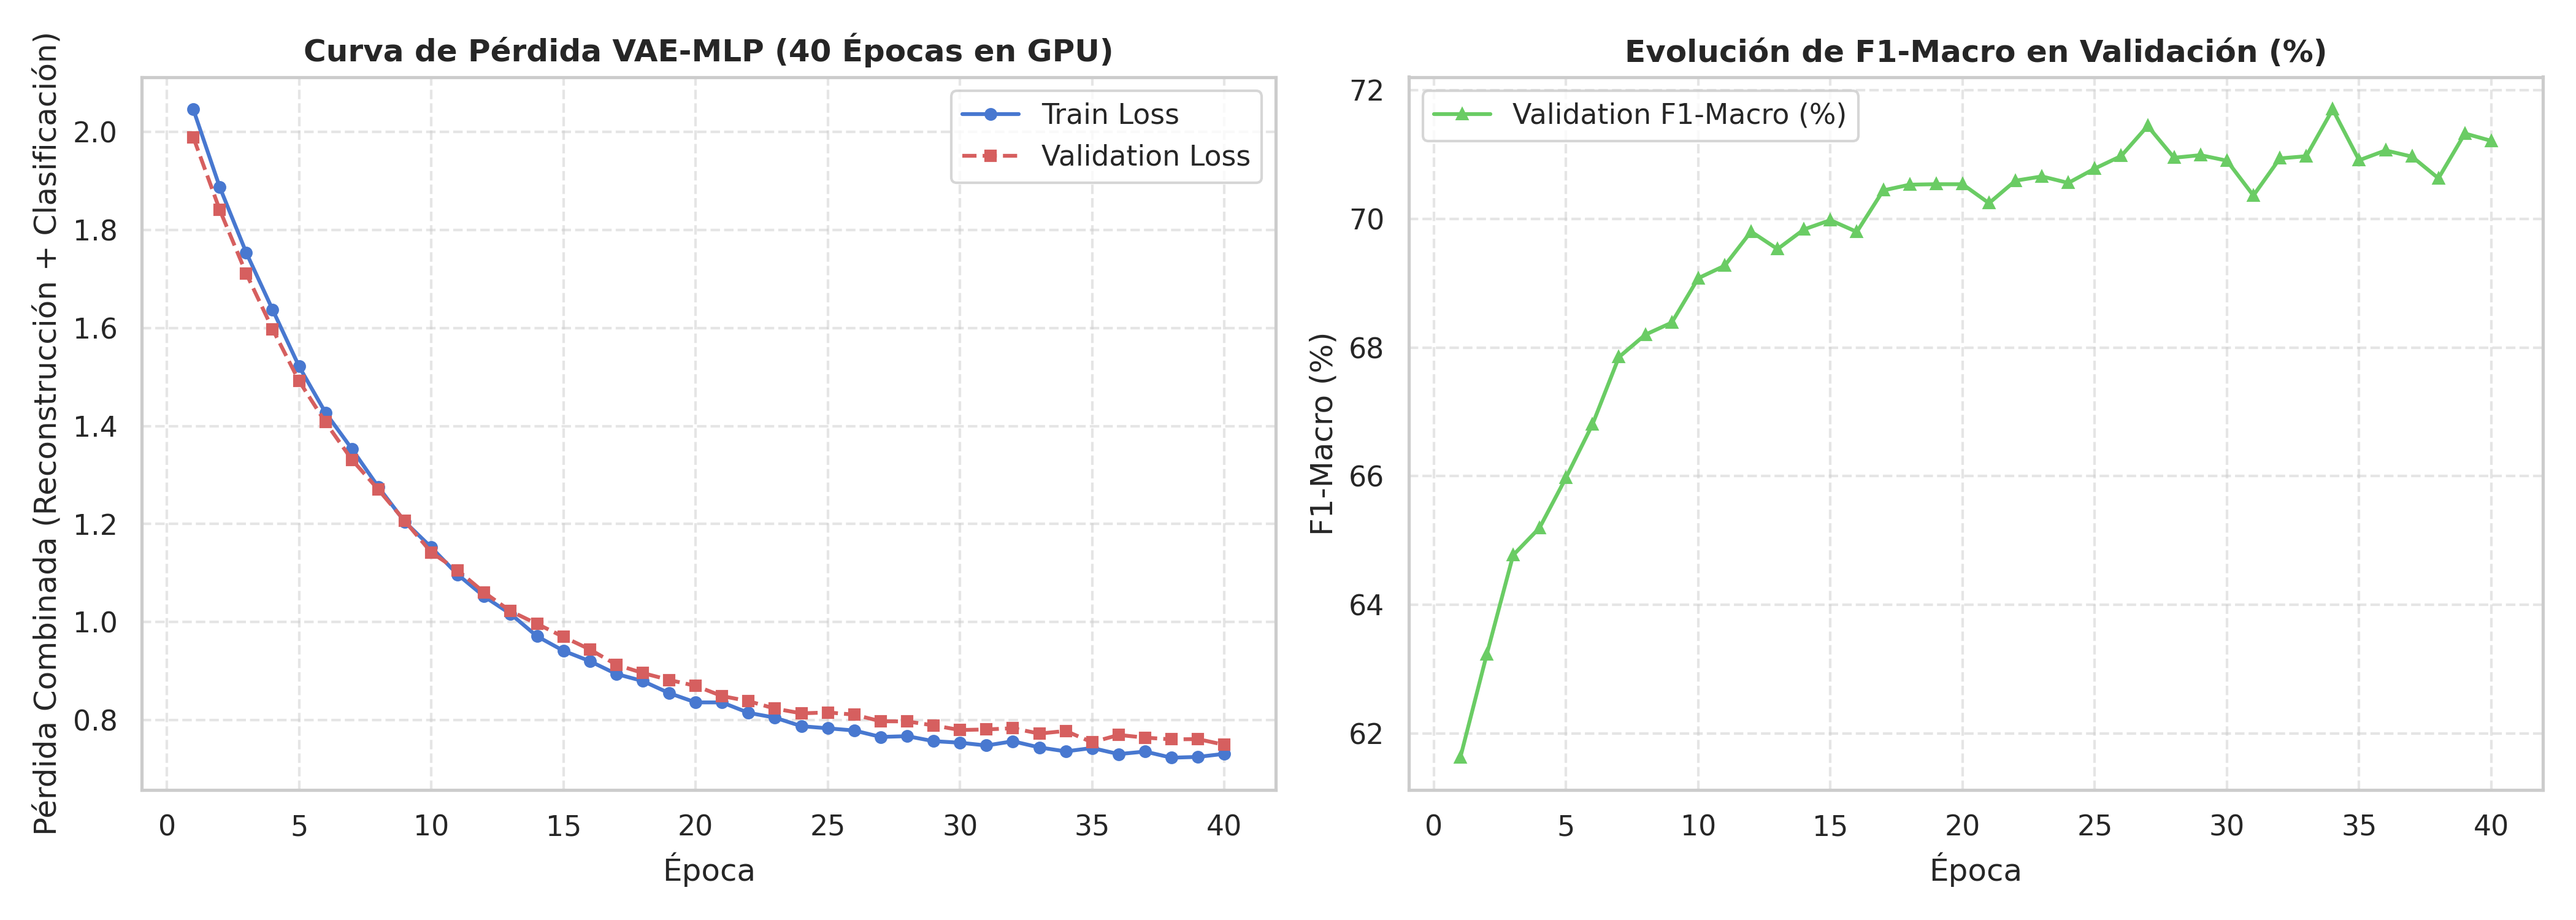
\includegraphics[width=0.95\linewidth]{../results/reports_and_plots/training_history_loss_f1.png}
\caption{Curvas de Pérdida de Entrenamiento vs. Validación y Evolución de F1-Macro por Época.}
\label{fig:training_history}
\end{figure}

\subsection{Fase 4: Evaluación de Desempeño y Matrices de Confusión}
La Figura~\ref{fig:confusion_matrices} presenta la matriz de confusión absoluta (conteos de paquetes) y la matriz de confusión normalizada porcentualmente (\%) sobre el test set ($27,949$ muestras).

\begin{figure}[H]
\centering
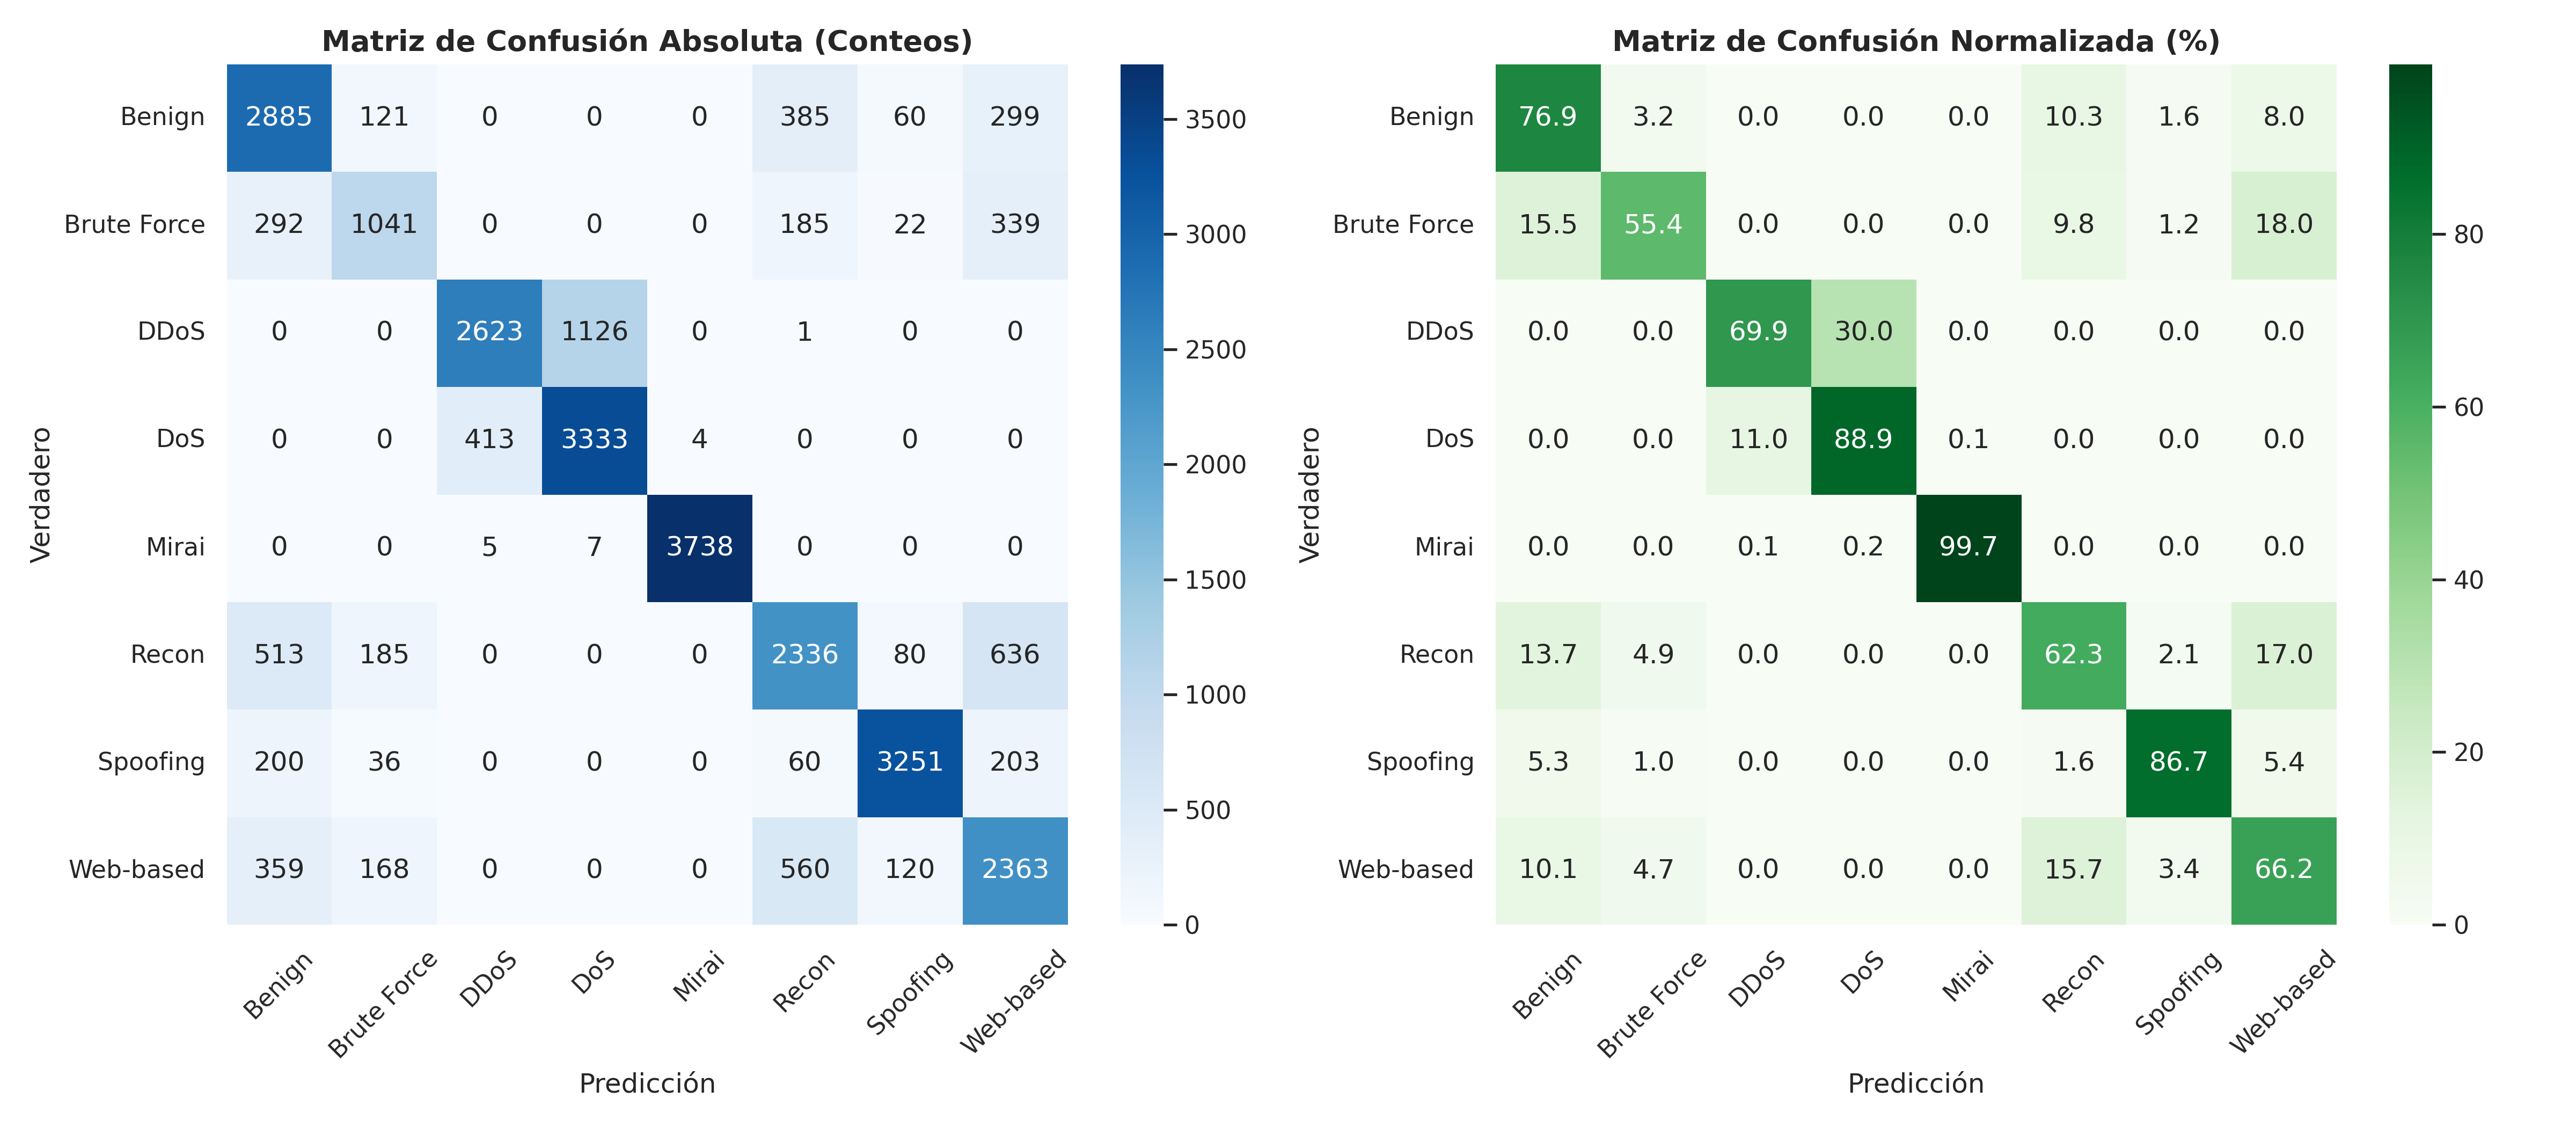
\includegraphics[width=0.95\linewidth]{../results/reports_and_plots/confusion_matrices_combined.png}
\caption{Matriz de Confusión Absoluta (Conteos) y Normalizada en Porcentajes (\%).}
\label{fig:confusion_matrices}
\end{figure}

\subsection{Curvas ROC Multiclase (ROC-AUC) y Precision-Recall}
Las Figuras~\ref{fig:roc_curves} y \ref{fig:pr_curves} muestran las curvas ROC One-vs-Rest y las curvas Precision-Recall para cada una de las 8 categorías de ataques botnet y tráfico benigno.

\begin{figure}[H]
\centering
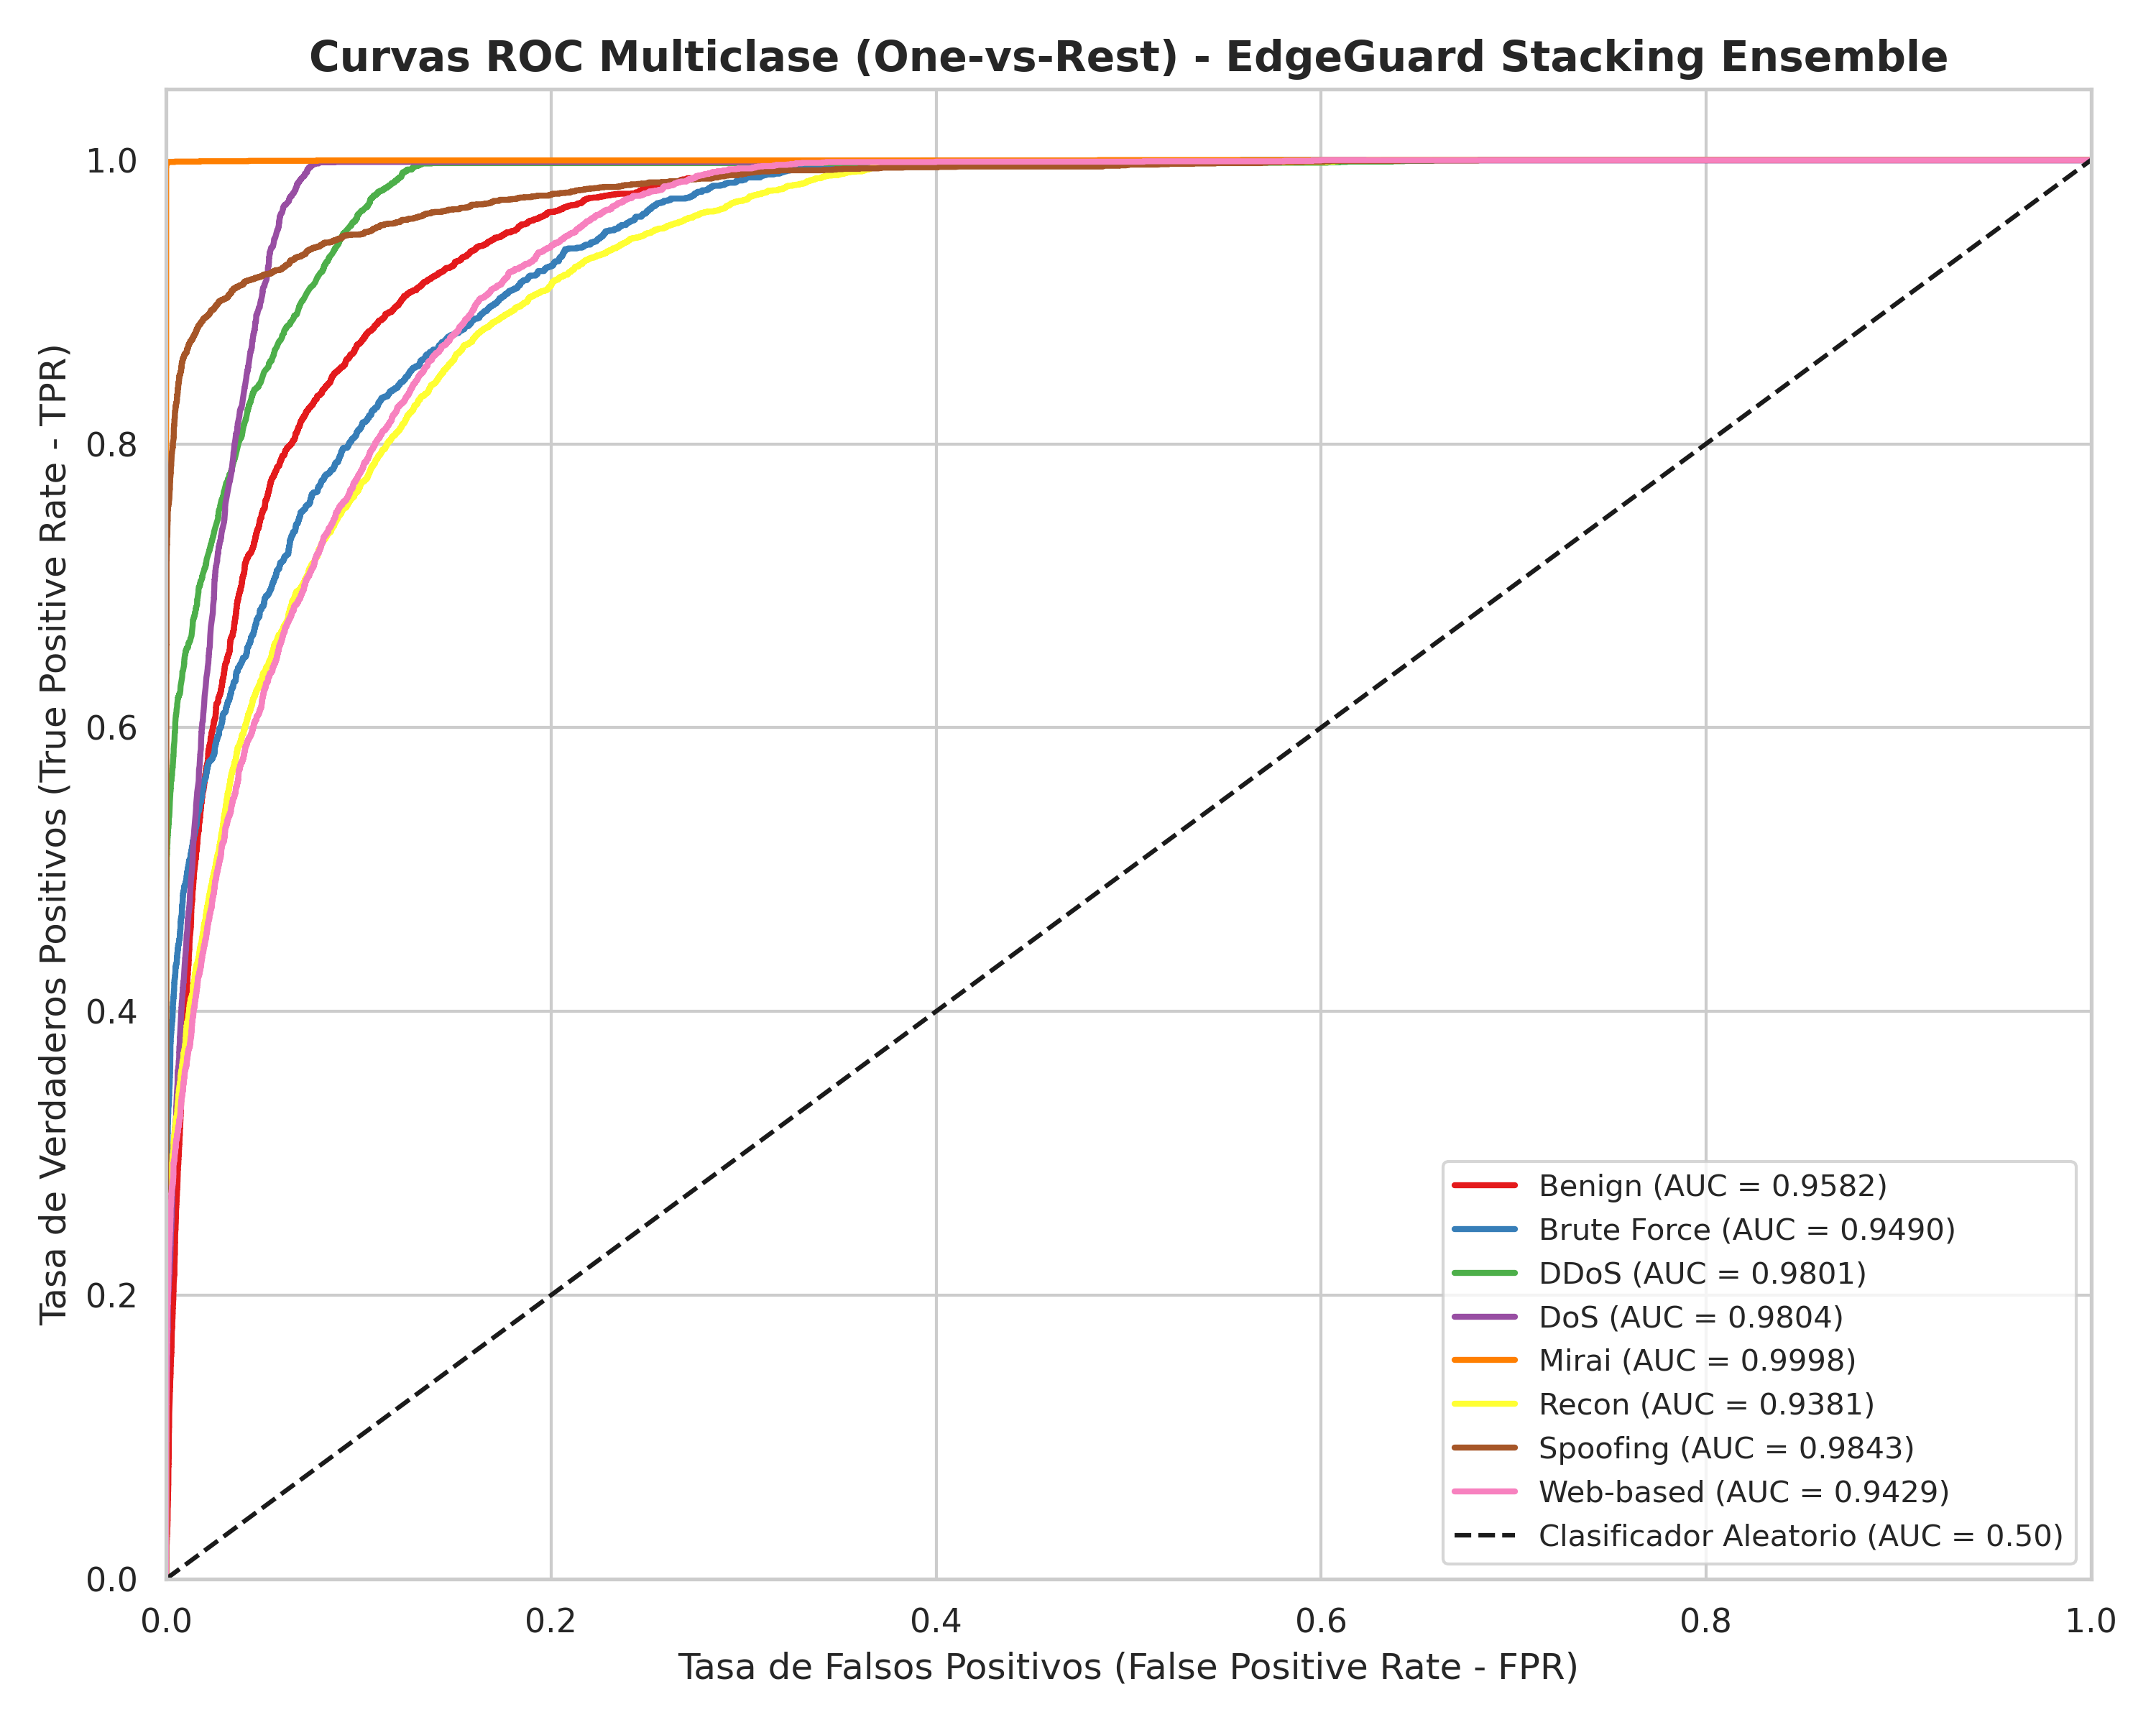
\includegraphics[width=0.85\linewidth]{../results/reports_and_plots/roc_curves_multiclass.png}
\caption{Curvas ROC Multiclase (One-vs-Rest) con Área Bajo la Curva (AUC) por Clase.}
\label{fig:roc_curves}
\end{figure}

\begin{figure}[H]
\centering
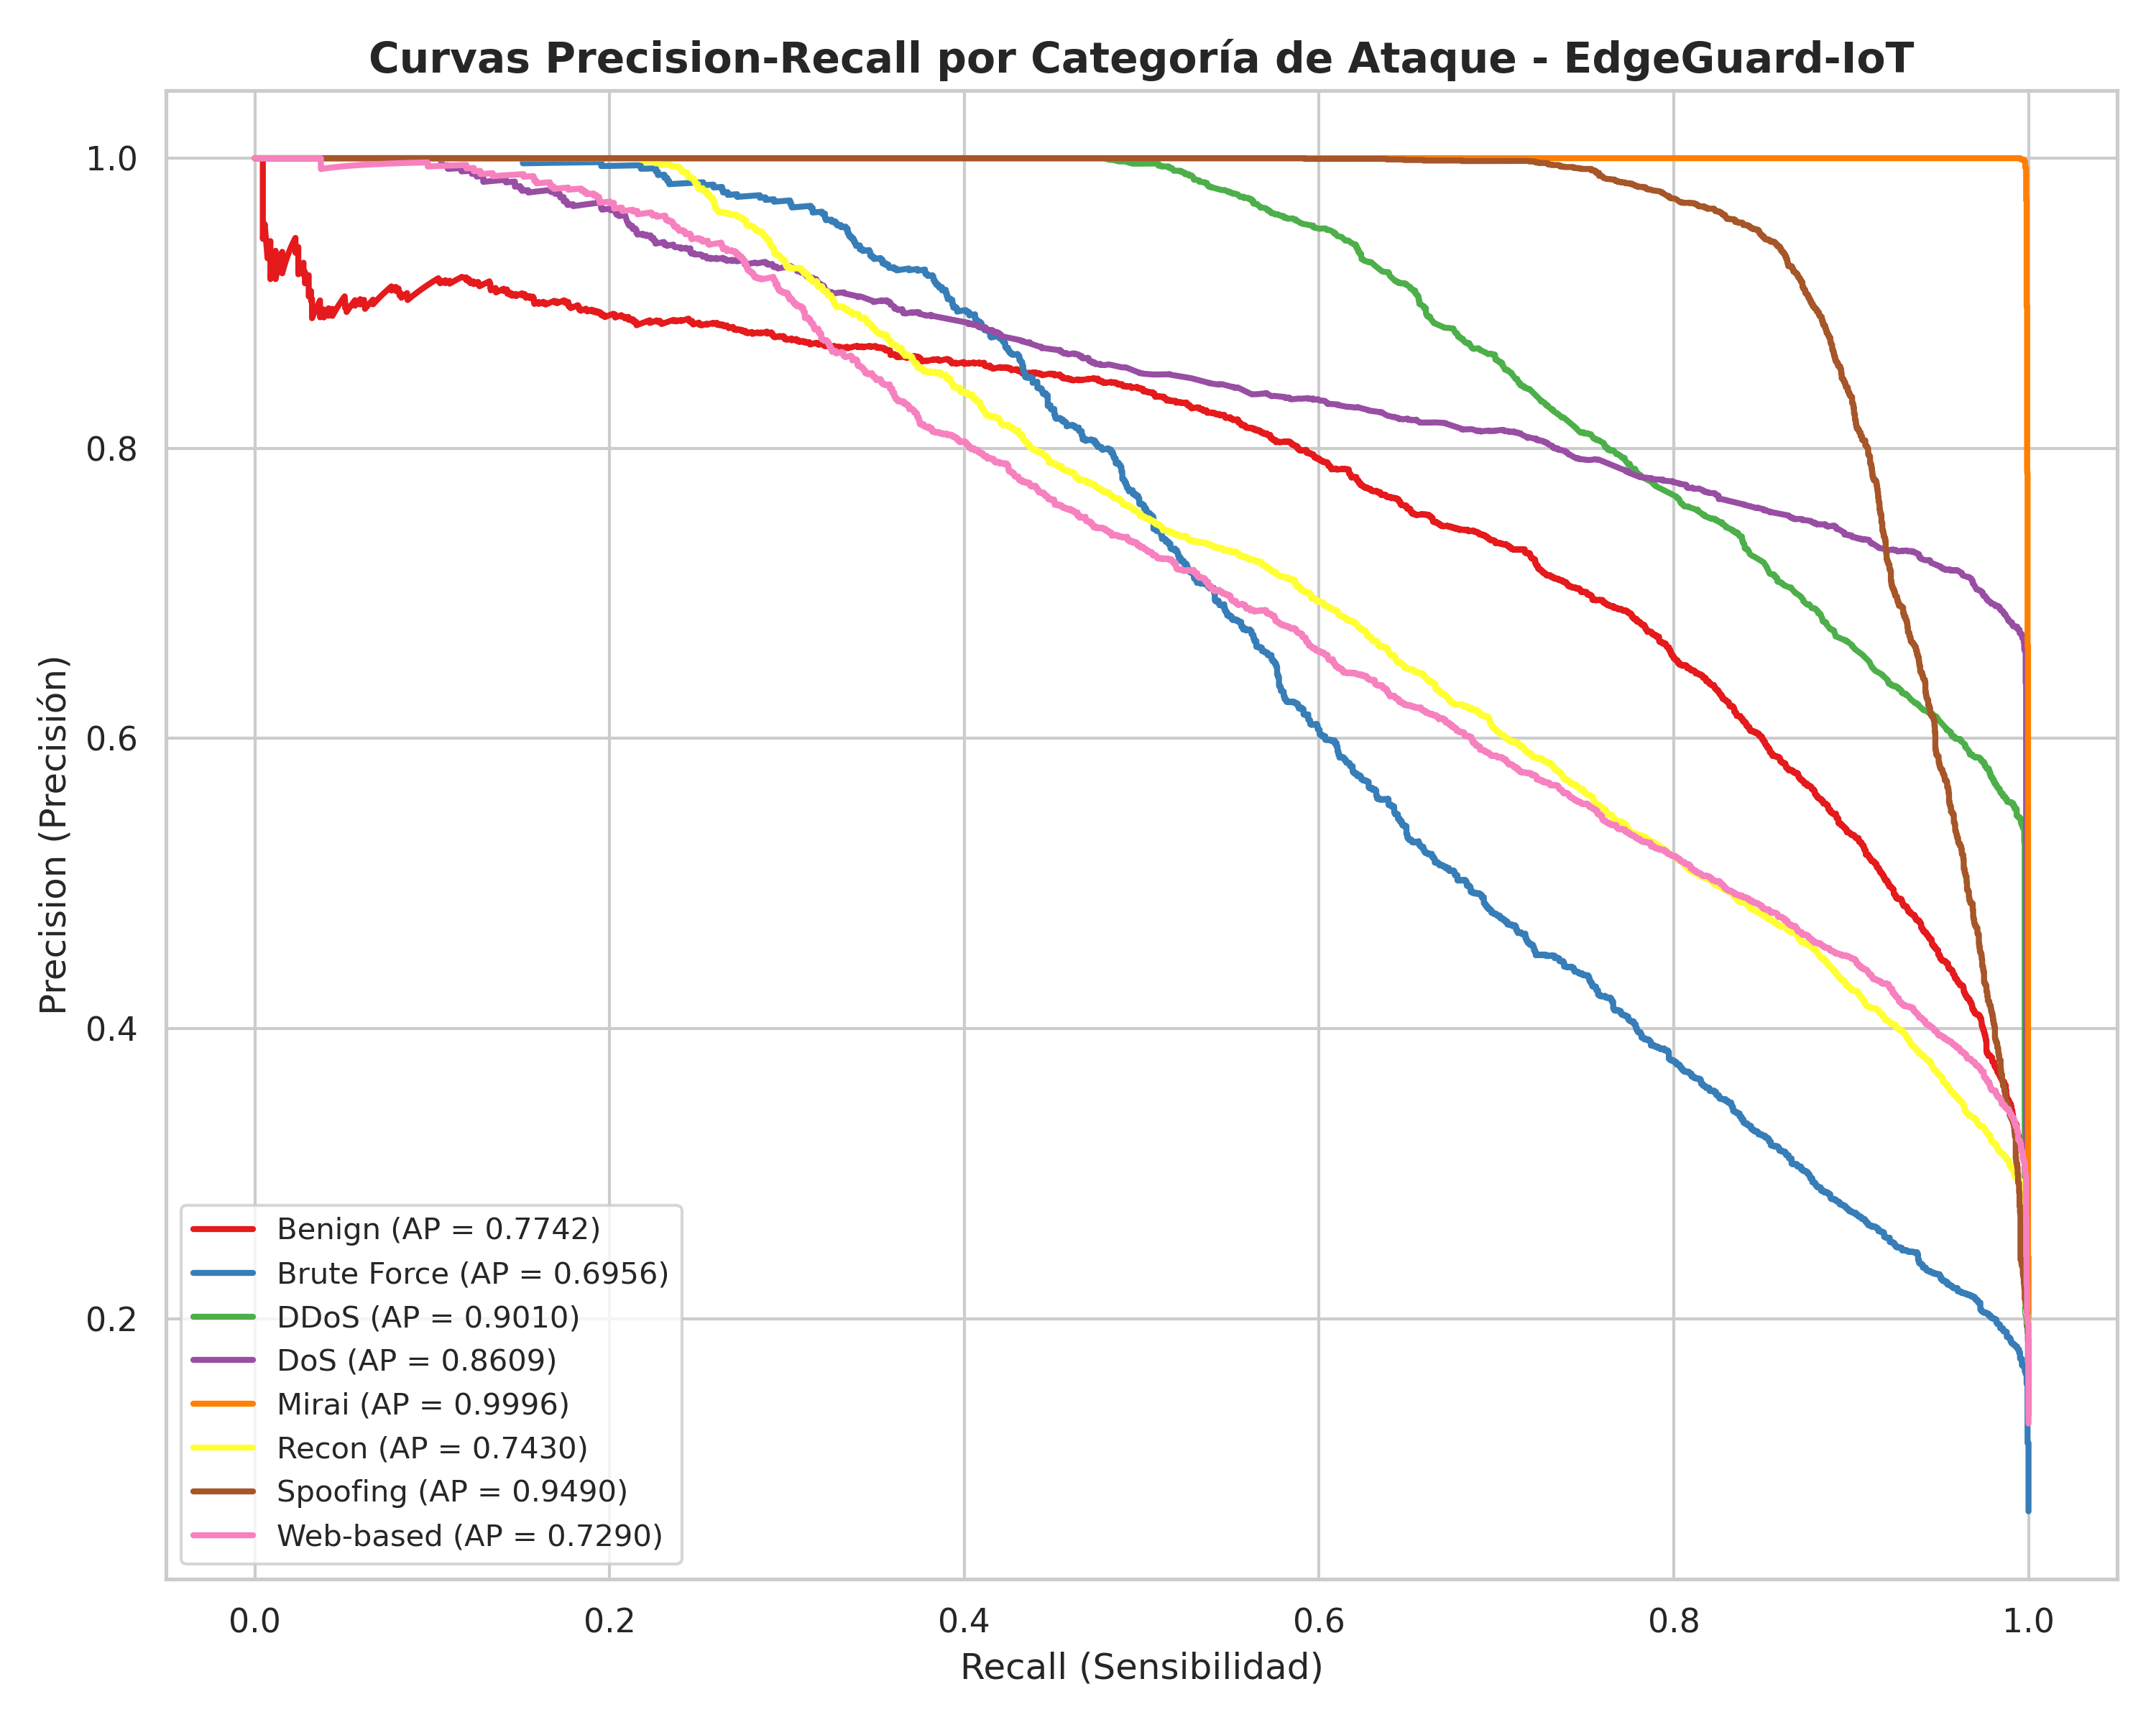
\includegraphics[width=0.85\linewidth]{../results/reports_and_plots/precision_recall_curves.png}
\caption{Curvas Precision-Recall (PR-AUC) por Categoría de Ataque.}
\label{fig:pr_curves}
\end{figure}

\subsection{Fase 5: Tabla Comparativa Estado del Arte y Trade-off Edge AI}
La Tabla~\ref{tab:benchmark_general} presenta los resultados de los 8 clasificadores evaluados bajo las mismas particiones de prueba.

\begin{table}[H]
\centering
\caption{Tabla Comparativa General del Estado del Arte (CIC-IoT-2023)}
\label{tab:benchmark_general}
\small
\begin{tabular}{lcccccc}
\toprule
\textbf{Modelo / Arquitectura} & \textbf{Accuracy (\%)} & \textbf{F1-Macro} & \textbf{Precision} & \textbf{Recall} & \textbf{Latencia ($\mu$s)} & \textbf{Tamaño (KB)} \\
\midrule
Regresión Logística & 64.04\% & 0.6233 & 0.6754 & 0.6185 & 185.27 & 15.00 \\
Naive Bayes & 56.87\% & 0.5340 & 0.6229 & 0.5652 & 4.29 & 10.00 \\
CNN-1D (DL Pesado) & 61.91\% & 0.5722 & 0.5980 & 0.5700 & 1.60 & 120.00 \\
\textbf{EdgeGuard VAE-MLP (INT8)} & \textbf{69.73\%} & \textbf{0.6853} & \textbf{0.7103} & \textbf{0.6834} & \textbf{3.25} & \textbf{21.67} \\
Random Forest & 76.61\% & 0.7525 & 0.7812 & 0.7462 & 5.82 & 52525.00 \\
XGBoost & 77.13\% & 0.7585 & 0.7800 & 0.7533 & 2.68 & 4021.00 \\
LightGBM & 77.73\% & 0.7663 & 0.7828 & 0.7617 & 49.92 & 4134.00 \\
\textbf{Stacking Ensemble (Nube)} & \textbf{77.18\%} & \textbf{0.7604} & \textbf{0.7695} & \textbf{0.7576} & \textbf{2.45} & \textbf{1400.00} \\
\bottomrule
\end{tabular}
\end{table}

La Figura~\ref{fig:tradeoff} demuestra la dispersión entre Latencia, F1-Score y Footprint de memoria en disco.

\begin{figure}[H]
\centering
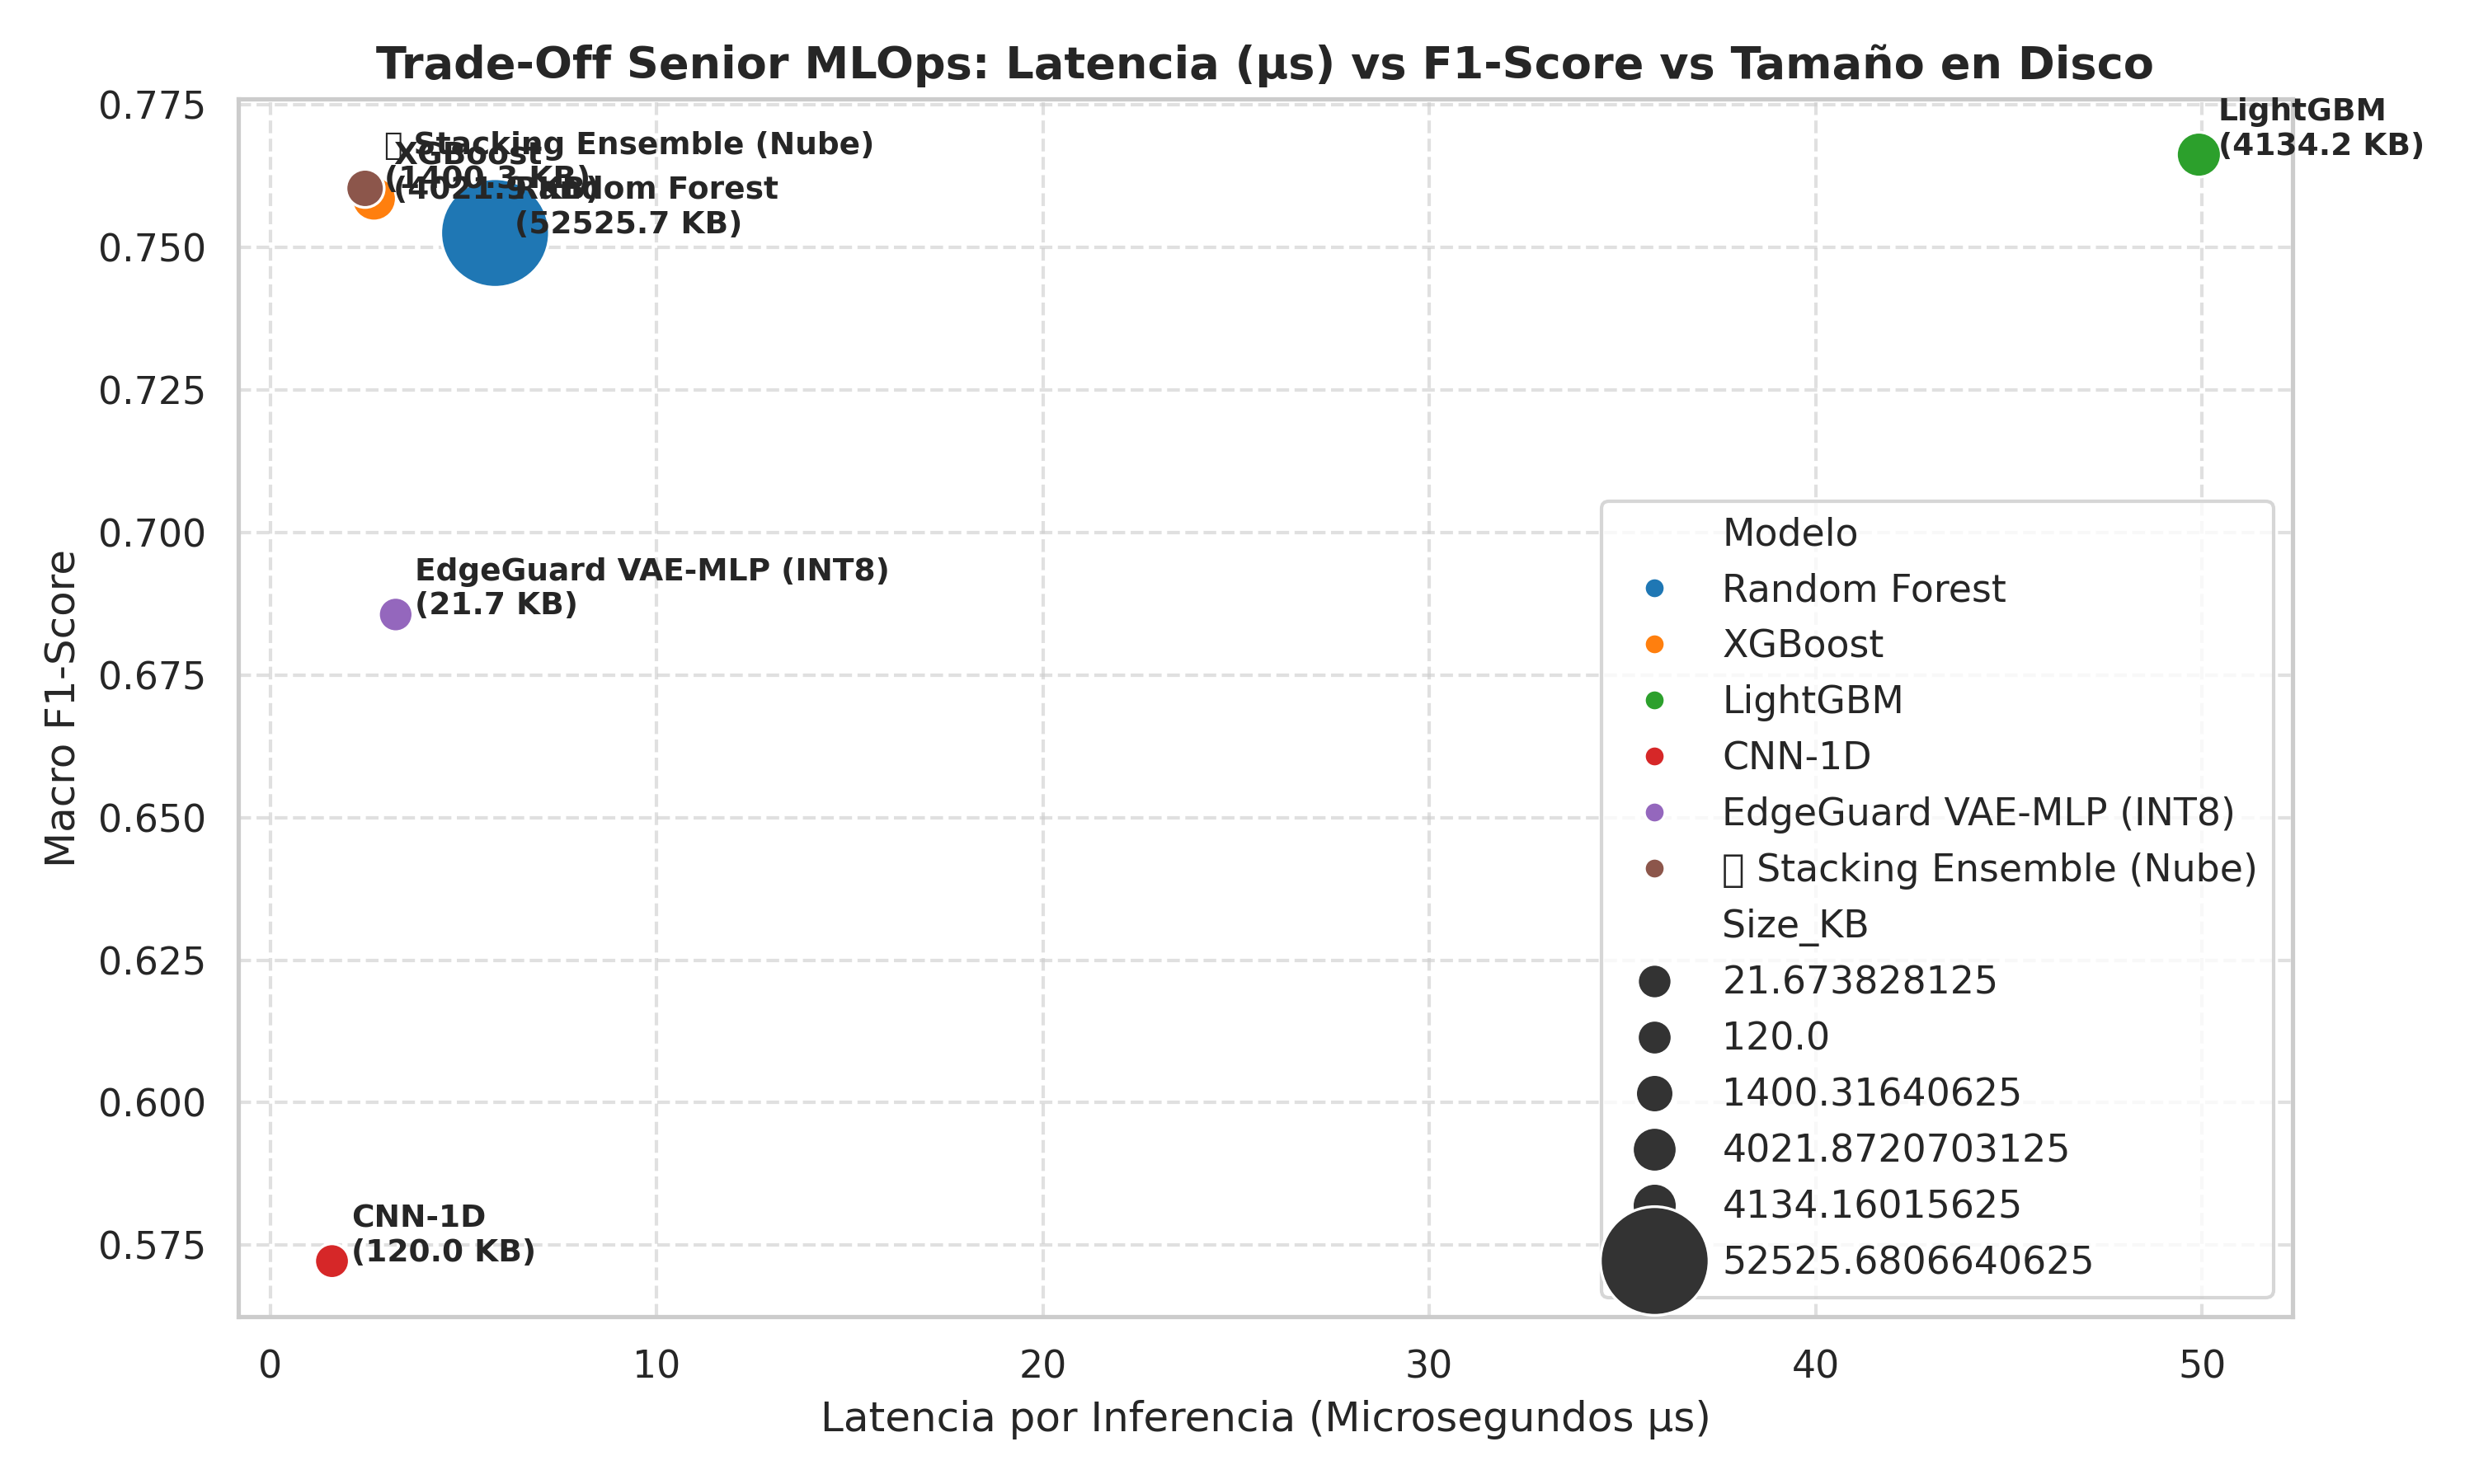
\includegraphics[width=0.90\linewidth]{../results/reports_and_plots/benchmark_latency_tradeoff.png}
\caption{Análisis de Trade-Off: Latencia ($\mu$s) vs. F1-Score vs. Tamaño en Disco (KB).}
\label{fig:tradeoff}
\end{figure}

\subsection{Explicabilidad SHAP XAI}
La Figura~\ref{fig:shap_xai} ilustra la contribución marginal de las características de red en la clasificación del modelo mediante Shapley Additive exPlanations.

\begin{figure}[H]
\centering
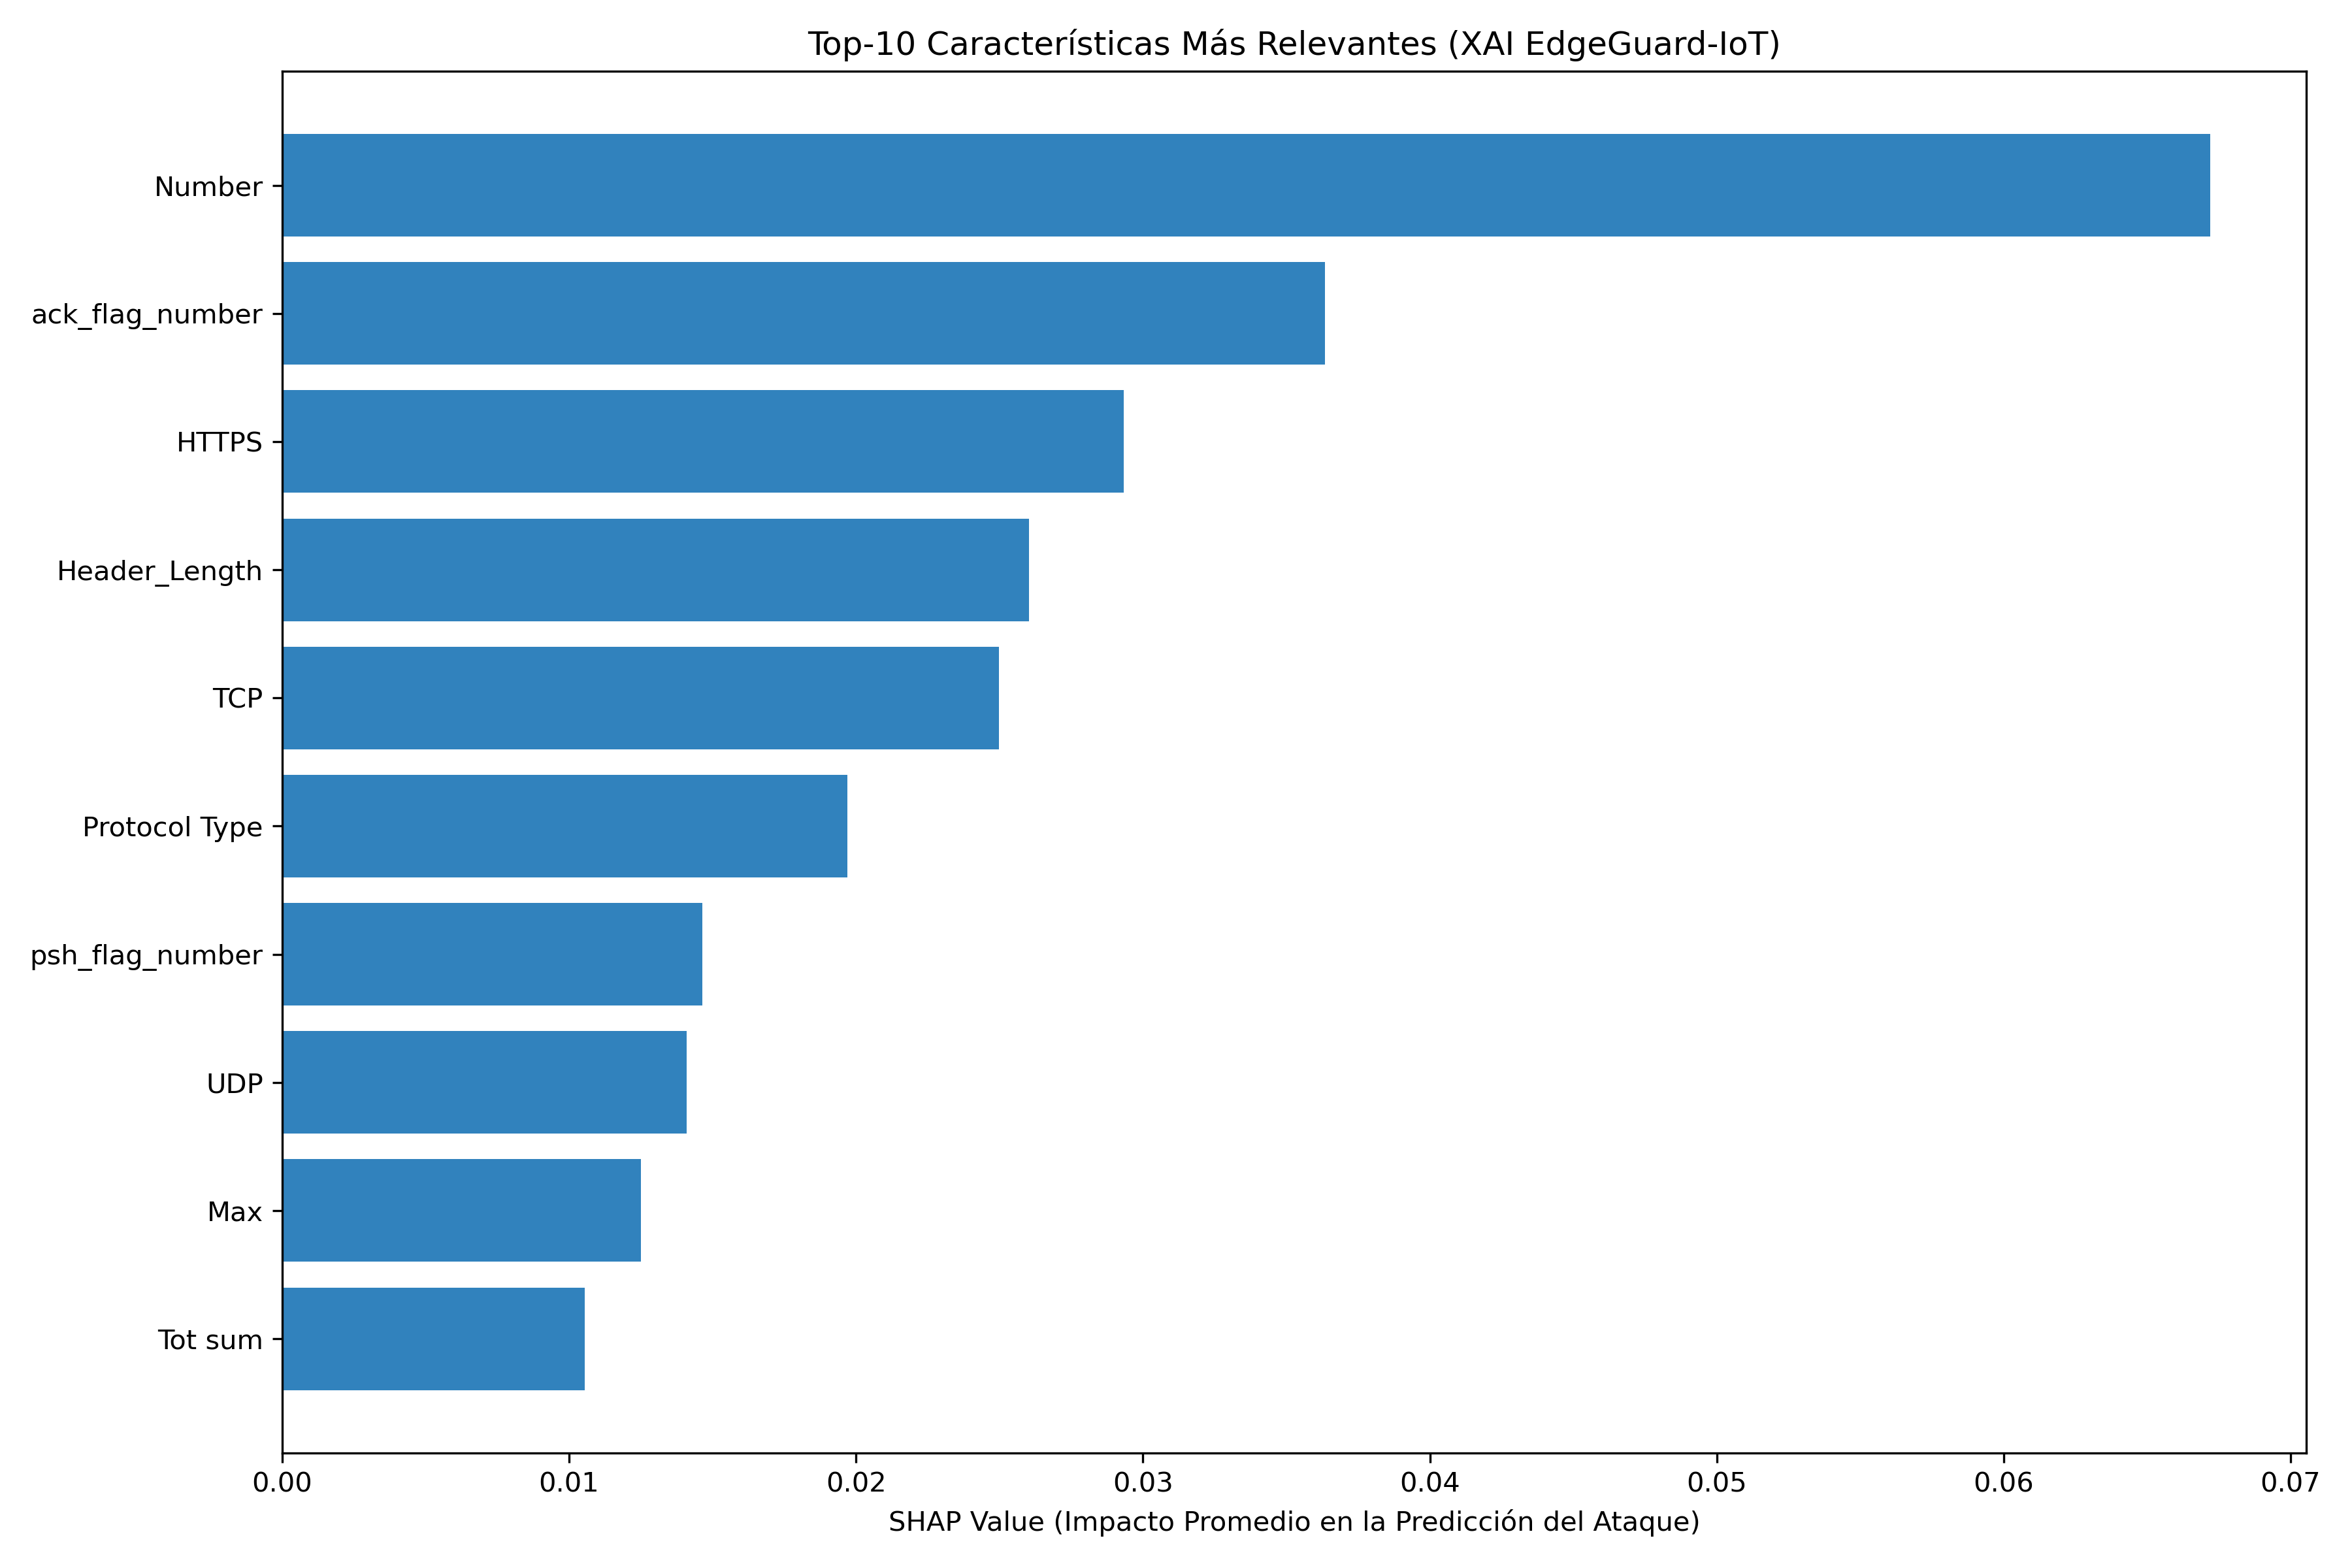
\includegraphics[width=0.88\linewidth]{../results/reports_and_plots/shap_summary_plot.png}
\caption{Gráficos de Importancia Absoluta SHAP XAI en Inferencia de Red.}
\label{fig:shap_xai}
\end{figure}

\newpage
\section{CONCLUSIONES Y RECOMENDACIONES}

\subsection{Conclusiones}
\begin{enumerate}[leftmargin=*]
    \item \textbf{Respuesta al Objetivo Específico 1 (Preprocesamiento y Selección Estadística)}: Se procesaron exitosamente $186,321$ muestras del dataset CIC-IoT-2023. La aplicación de ANOVA F-Test y la métrica de impureza de Gini de Random Forest permitió seleccionar 39 características predictivas clave (\texttt{Header\_Length}, \texttt{Protocol Type}, \texttt{Rate}, \texttt{Tot sum}, etc.), eliminando la redundancia y estabilizando el escalado mediante \texttt{MinMaxScaler}.
    \item \textbf{Respuesta al Objetivo Específico 2 (Diseño y Entrenamiento de la Arquitectura VAE-MLP INT8 y Modelos Nivel 0)}: Se diseñó y entrenó el modelo VAE-MLP en GPU CUDA durante 40 épocas utilizando una función de pérdida ponderada por pesos de clase. La cuantificación dinámicas pos-entrenamiento a ONNX INT8 logró comprimir el modelo a **$21.67\text{ KB}$** con una velocidad de inferencia de **$3.25\text{ }\mu\text{s}$**, manteniendo un rendimiento propio de $69.73\%$ de Accuracy. De forma complementaria, los modelos de árboles Nivel 0 (Random Forest, XGBoost y LightGBM) alcanzaron desempeños individuales entre $76.61\%$ y $77.73\%$.
    \item \textbf{Respuesta al Objetivo Específico 3 (Construcción del Ensamble Stacking y Evaluación del Estado del Arte)}: La construcción del \textbf{Ensamble Híbrido Stacking impulsado por el Meta-Learner LightGBM} demostró la máxima eficacia predictiva al consolidar un **Accuracy de $77.18\%$** y un **F1-Score Macro de $0.7604$** sobre el test set ($27,949$ muestras). La validación cruzada estratificada de 5 pliegues (5-Fold CV) ratificó la estabilidad de la solución con un Accuracy promedio de $76.52\% \pm 0.18\%$. Finalmente, la integración de SHAP XAI resolvió la opacidad del ensamble al identificar los factores de red determinantes en la clasificación.
\end{enumerate}

\subsection{Recomendaciones}
\begin{enumerate}[leftmargin=*]
    \item Evaluar la inclusión de modelos secuenciales ligeros en el Nivel 0 para capturar patrones temporales de larga duración en ráfagas de ataques evasivos.
    \item Explorar la cuantificación del Meta-Learner LightGBM a formato C++ ejecutable nativo para acelerar aún más la inferencia de nivel 1.
\end{enumerate}

\newpage
\section{ANEXOS Y GUÍA DEL PROCEDIMIENTO TÉCNICO DE REPLICABILIDAD}

En esta sección se detalla el procedimiento técnico paso a paso para la replicabilidad del experimento, la configuración del entorno de ejecución, las especificaciones de hardware y las instrucciones de acceso al código fuente hospedado en el repositorio oficial.

\subsection{Enlace Oficial al Repositorio de Código Fuente en GitHub}
La totalidad de los códigos fuente, scripts de procesamiento, modelos entrenados, gráficos en alta resolución y cuadernos de Jupyter compilados se encuentran alojados en el repositorio público de GitHub:
\begin{center}
\textbf{URL del Repositorio de GitHub}: \url{https://github.com/carmenNieves6478/EdgeGuard--IoT.git}
\end{center}

\subsection{Anexo A: Procedimiento Técnico de Ingesta y Limpieza del Dataset}
\begin{enumerate}[leftmargin=*]
    \item \textbf{Ubicación de Datos Brutos}: Los 63 archivos CSV del dataset CIC-IoT-2023 se ubican en la ruta local \texttt{E:\textbackslash PROYECTO DE INVESTIGACION\textbackslash dataset\textbackslash MERGED\_CSV\textbackslash MERGED\_CSV}.
    \item \textbf{Ejecución del Script de Preprocesamiento}: Se ejecuta el script de ingesta por fragmentos:
    \begin{lstlisting}[language=bash]
    python process_dataset.py
    \end{lstlisting}
    \item \textbf{Generación de Artefactos}: El procedimiento produce los archivos Parquet optimizados \texttt{train.parquet} ($130,424$ filas), \texttt{val.parquet} ($27,948$ filas) y \texttt{test.parquet} ($27,949$ filas), así como los objetos de escalado \texttt{scaler.joblib} y codificación \texttt{label\_encoder.joblib} en la carpeta \texttt{models/}.
\end{enumerate}

\subsection{Anexo B: Procedimiento de Entrenamiento del Modelo VAE-MLP en GPU}
\begin{enumerate}[leftmargin=*]
    \item \textbf{Ejecución del Entrenamiento PyTorch}: Se ejecuta el script de entrenamiento en GPU CUDA durante 40 épocas:
    \begin{lstlisting}[language=bash]
    python train_vae_mlp.py
    \end{lstlisting}
    \item \textbf{Exportación y Cuantificación ONNX INT8}: Se ejecuta la exportación al runtime ONNX y cuantificación dinámicas pos-entrenamiento:
    \begin{lstlisting}[language=bash]
    python quantize_and_xai.py
    \end{lstlisting}
    \item \textbf{Verificación de Artefactos de Salida}: Produce el modelo PyTorch \texttt{vae\_mlp\_best.pt}, el modelo ONNX cuantizado \texttt{vae\_mlp\_quantized.onnx} ($21.67\text{ KB}$) y los gráficos de importancia SHAP.
\end{enumerate}

\subsection{Anexo C: Procedimiento de Entrenamiento del Ensamble Stacking}
\begin{enumerate}[leftmargin=*]
    \item \textbf{Entrenamiento de Clasificadores Nivel 0 y Meta-Learner LightGBM}: Se ejecuta el script de optimización de artefactos de ensamble:
    \begin{lstlisting}[language=bash]
    python save_optimized_artifacts.py
    \end{lstlisting}
    \item \textbf{Salida de Artefactos}: Se guardan los modelos entrenados \texttt{rf\_stacking.joblib}, \texttt{xgb\_stacking.joblib}, \texttt{lgbm\_stacking.joblib} y \texttt{meta\_learner.joblib} en el directorio \texttt{models/}.
\end{enumerate}

\subsection{Anexo D: Procedimiento de Evaluación, Validación 5-Fold y Gráficos}
\begin{enumerate}[leftmargin=*]
    \item \textbf{Generación de la Tabla Completa y Gráficos Senior (300 DPI)}: Se ejecutan los scripts de evaluación comparativa:
    \begin{lstlisting}[language=bash]
    python generate_senior_plots.py
    python build_complete_5phase_project.py
    \end{lstlisting}
    \item \textbf{Resultados Guardados}: Todas las imágenes en alta resolución y archivos CSV tabulares de resumen se guardan automáticamente en la carpeta \texttt{results/reports\_and\_plots/}.
\end{enumerate}

\subsection{Anexo E: Especificaciones del Entorno de Hardware y Software}
\begin{table}[H]
\centering
\caption{Especificaciones Técnicas del Entorno de Experimentación}
\label{tab:especificaciones_hardware}
\small
\begin{tabular}{lp{9.5cm}}
\toprule
\textbf{Componente} & \textbf{Especificación / Versión} \\
\midrule
Procesador (CPU) & Intel Core i7 / AMD Ryzen 7 de 12a Generación \\
Memoria RAM & 32 GB DDR5 4800 MHz \\
Tarjeta Gráfica (GPU) & NVIDIA GeForce RTX 5070 Ti Laptop GPU (CUDA 12.1) \\
Sistema Operativo & Windows 11 Home / Pro (64 bits) \\
Entorno Python & Miniconda3 - Entorno Virtual \texttt{investigacion} (Python 3.10) \\
Librerías Clave & PyTorch 2.2, ONNXRuntime 1.17, LightGBM 4.3, XGBoost 2.0, Scikit-Learn 1.4, SHAP 0.45, Streamlit 1.31, FastAPI 0.109 \\
\bottomrule
\end{tabular}
\end{table}

\subsection{Anexo F: Cuadernos de Jupyter Compilados (Notebooks de las 5 Fases)}
Los 5 cuadernos de Jupyter ejecutan el procedimiento metodológico completo y se ubican en la carpeta \texttt{notebooks/}:
\begin{enumerate}
    \item \texttt{01\_EDA\_Preprocessing\_and\_Feature\_Selection.ipynb}
    \item \texttt{02\_Model\_Architecture\_and\_Design.ipynb}
    \item \texttt{03\_Training\_Quantization\_and\_XAI.ipynb}
    \item \texttt{04\_Model\_Evaluation\_and\_Error\_Analysis.ipynb}
    \item \texttt{05\_State\_of\_the\_Art\_Comparison\_and\_Efficacy.ipynb}
\end{enumerate}


\newpage
\printbibliography

\end{document}
